%%%%%%%%%%%%%%%%%%%%%%%%%%%%%%%%%%%%%%%%%%%%%%%%%%%
%
%  New template code for TAMU Theses and Dissertations starting Fall 2016.  
%
%
%  Author: Sean Zachary Roberson
%  Version 3.17.09
%  Last Updated: 9/21/2017
%
%%%%%%%%%%%%%%%%%%%%%%%%%%%%%%%%%%%%%%%%%%%%%%%%%%%
%%%%%%%%%%%%%%%%%%%%%%%%%%%%%%%%%%%%%%%%%%%%%%%%%%%%%%%%%%%%%%%%%%%%%%
%%                           SECTION III
%%%%%%%%%%%%%%%%%%%%%%%%%%%%%%%%%%%%%%%%%%%%%%%%%%%%%%%%%%%%%%%%%%%%%

\chapter{ \uppercase{Numerical Examples}}

In the following examples I explore the advantages of the GFEM approach when compared to the standard FEM regarding accuracy and simulation time for some relevant cases in exploration seismology. In these examples I use a model in $R^2$ whose dimensions are 800 m in the horizontal direction and 400 m in the vertical direction except for the last case for which I include some topographic relief. I also include a seismic source as defined in equation \ref{Eq2.15} with a central frequency $f_o=$40 Hz. For every example I find a reference solution in a fine mesh applying the standard FEM, and compare the performance against various GFEM simulation cases, presenting error estimates versus simulation time. I also find additional solutions with the standard FEM for coarser meshes to compare the overall performance against the GFEM technique. 

From the second seismic model on-wards I show the corresponding shot gathers in a variable density presentation (See Figures \ref{fig:3.15}, \ref{fig:3.27} and  \ref{fig:3.41}). For all these figures the amplitude of the traces have been modified by incorporating a time dependent divergence correction and by applying a fixed gain to each trace with the purpose of enhancing data visualization.

To find the divergence corrected traces I use the following equation:
 \begin{equation} \label{Eq3.1}
  T_d(t) = T(t)\, t^\alpha
 \end{equation}
Where  $T_d(t)$ is the divergence-corrected trace,$T(t)$ is the trace to modify, $t$ is time and $\alpha$ is a user defined factor. Since the purpose of this correction is to enhance later arrivals, $\alpha$ is commonly greater than 1.

The fixed gain is applied as follows:
 \begin{equation} \label{Eq3.2}
  Tg_i(t) = \frac{mx}{mx_i}\, T_i(t)
 \end{equation}
Where $Tg_i(t)$ is the i-th gain-modified trace of a shot gather, $Tg_i(t)$ is the corresponding input trace, $mx$ is the maximum amplitude of the shot gather and $mx_i$ is the maximum amplitude of the corresponding trace.

All other figures showing individual traces correspond to raw data without any further modification.

\section{Case 1: Homogeneous Medium}
For this case, I  assume that the medium has an acoustic velocity of 1800 m/s. I  place a seismic source at the center of the model, I also locate receivers in a radial configuration at 50 m and 100 m from the center of the source, with a receiver spacing of 5 degrees as shown in Figure \ref{fig:3.1}. The reference solution corresponds to a fine mesh with grid size $h=$1.5625 m and source radius of $2h$. For all the GFEM cases the wave number used for the plane wave enrichments is 0.14 m$^{-1}$, calculated by dividing the source radial frequency by the medium velocity.

 \begin{figure}[h!]
	\centering
	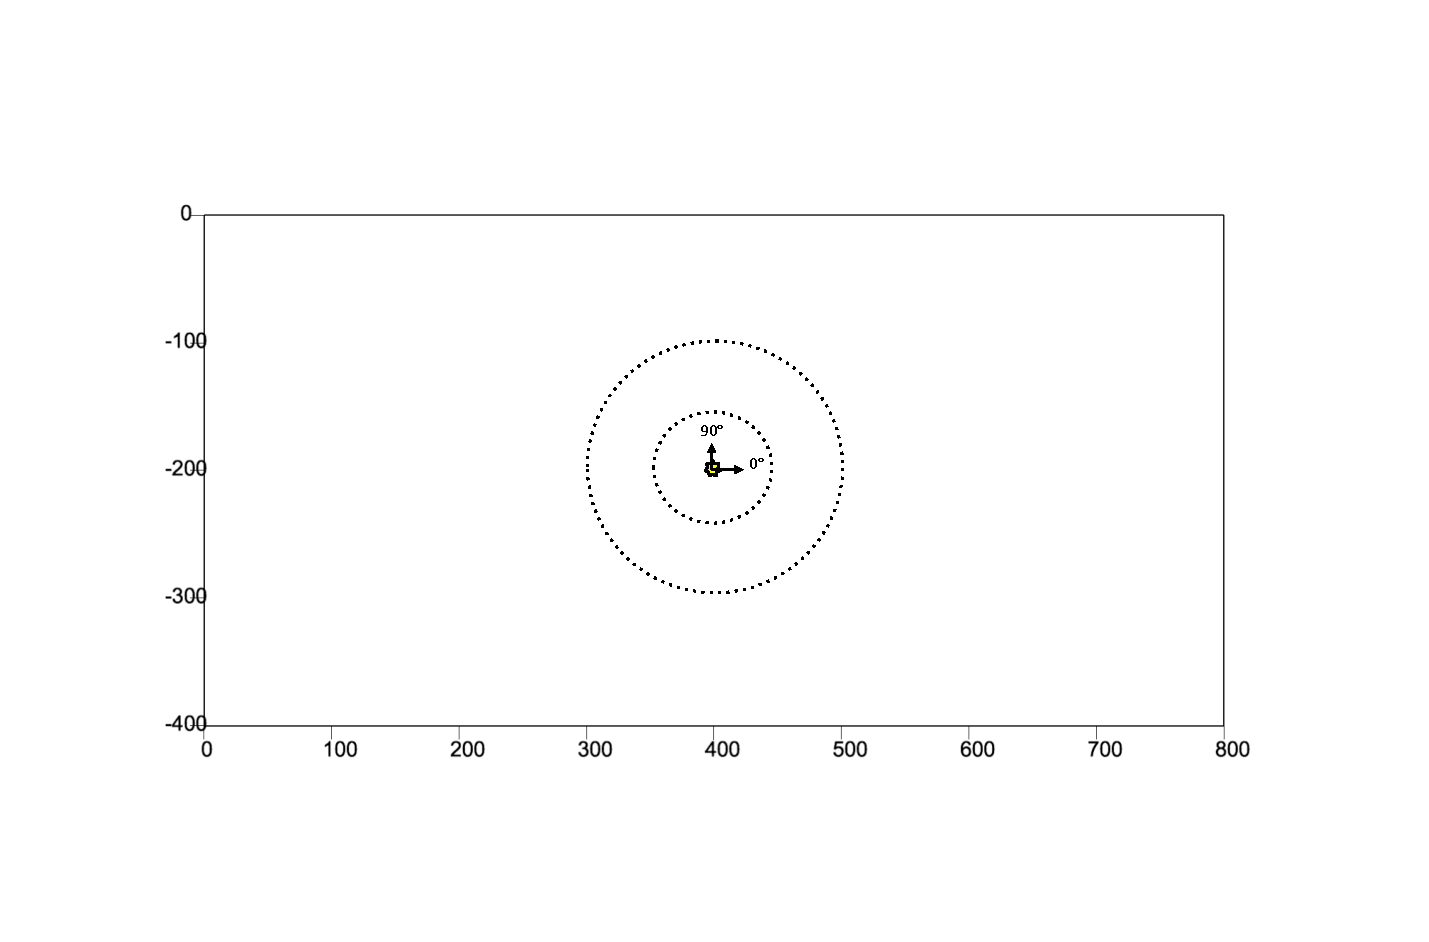
\includegraphics[width=12cm, height=6.5cm]{Thesis_Edith/figures/homo/h_source.pdf}
	\caption{Homogeneous model with a seismic source in the center (yellow star) and two sets of receiver arrays (dotted circles) at 50 m and at 100 m from the center of the source.}
	\label{fig:3.1}
\end{figure}

\clearpage
\subsection{Effect of Source Size}
%GFEM
%********************
Since I am using a source with a finite dimension for these simulations, I investigate the effect of source size on the accuracy of the GFEM solutions. Figure \ref{fig:3.2} and Figure \ref{fig:3.3} show the effect of source radius on the simulated seismograms obtained with the GFEM approach. For these cases, I used source radii equal to the mesh size and smaller than the mesh size. The plots show that to obtain the best solution approximation the source radius should be at least equal (or greater) to the mesh size as depicted in Figure \ref{fig:3.4}.

 \begin{figure}[h!]
 		\centering
		\begin{subfigure}{8cm}
				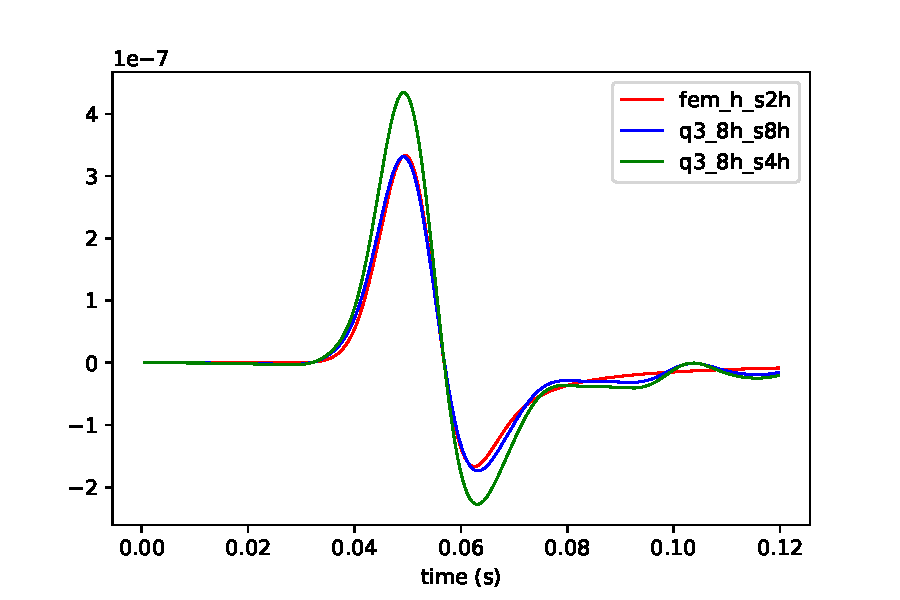
\includegraphics[width=8 cm, height=5.5cm]{Thesis_Edith/figures/homo/homo_waves/fem_q3_8h_r50_0deg.pdf} 
			     \caption{}
				%\label{fig:trace1}
		\end{subfigure}
        \hspace{0.25cm}
		\begin{subfigure}{8cm}
				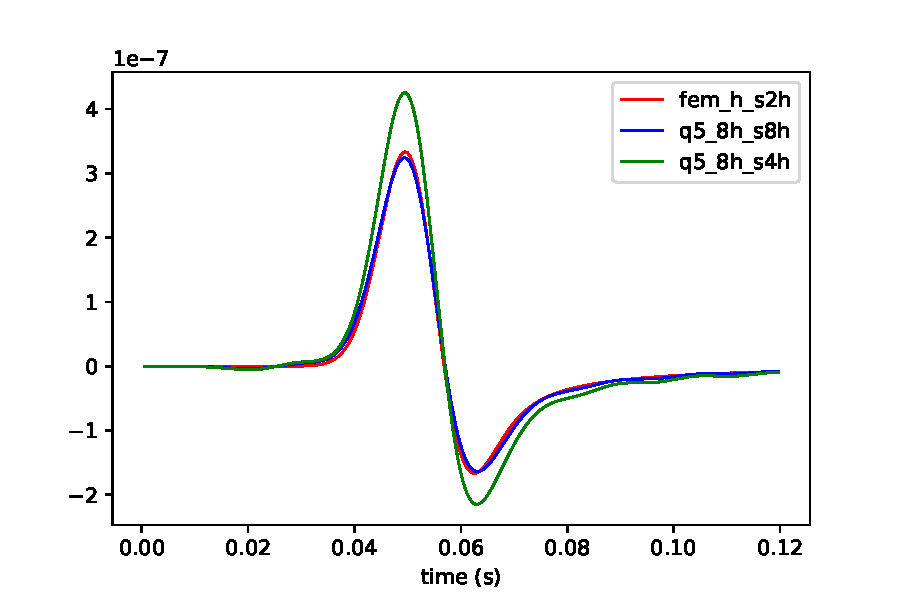
\includegraphics[width=8cm, height=5.5cm]{Thesis_Edith/figures/homo/homo_waves/fem_q5_8h_r50_0deg.pdf}
			   \caption{}
				%\label{fig:trace3}
		\end{subfigure}
 
	\caption{Homogeneous model: Seismograms for a receiver at 0 deg and  50 m from the source center  (see Figure \ref{fig:3.1}). GFEM solutions correspond to a mesh size of $8h$ and source radius of  $8h$ and $4h$. (a) Seismograms for the reference solution and 2 GFEM solutions with plane waves in 3 directions. (b) Seismograms showing the reference solution and 2 GFEM solutions with plane waves in 5 directions.}
	\label{fig:3.2}
\end{figure}


 \begin{figure}[h!]
 		\centering
		\begin{subfigure}{8cm}
				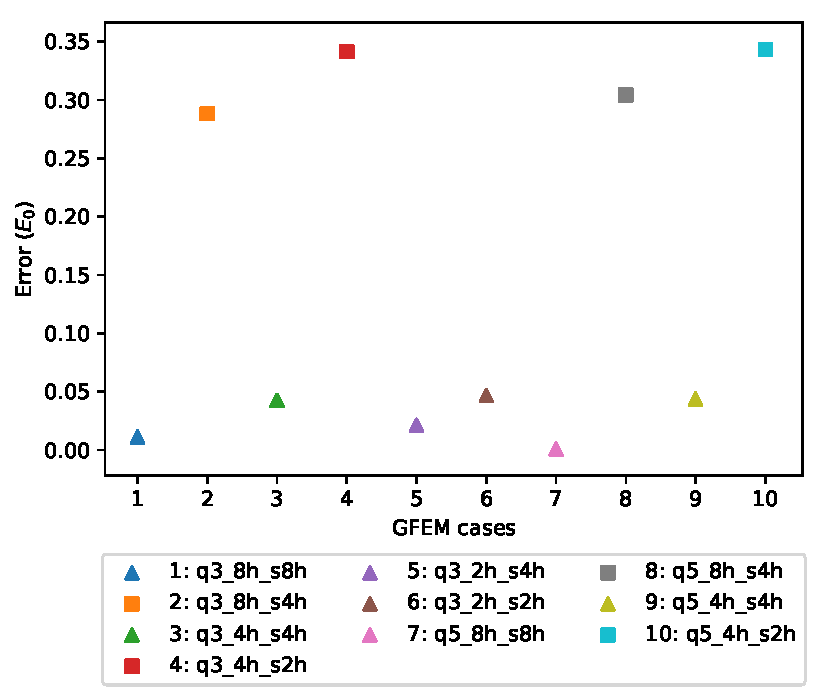
\includegraphics[width=8cm, height=6cm]{Thesis_Edith/figures/homo/homo_waves/error_gfem_50m.pdf} 
			     \caption{}
				%\label{fig:trace1}
		\end{subfigure}
        \hspace{0.25cm}
		\begin{subfigure}{8cm}
				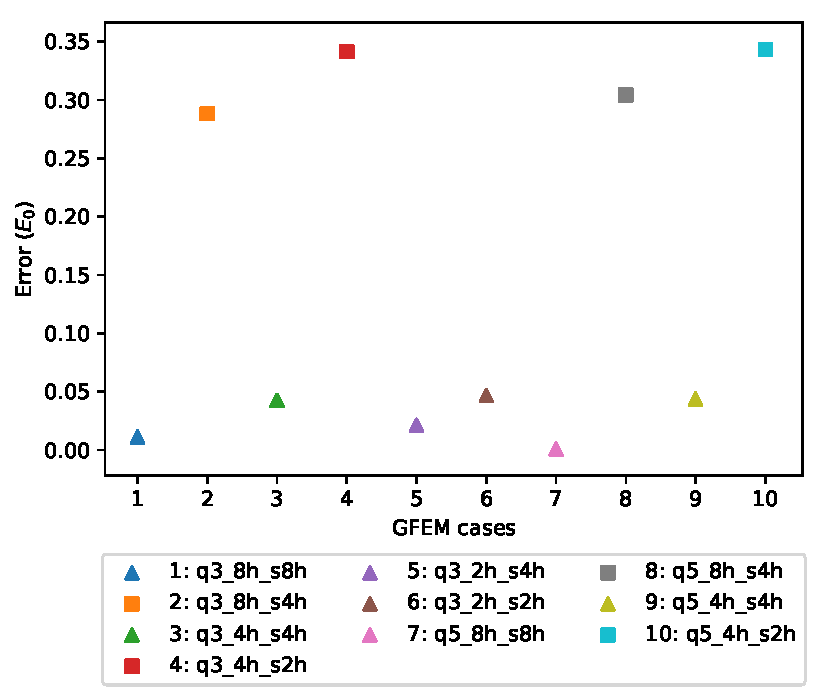
\includegraphics[width=8cm, height=6cm]{Thesis_Edith/figures/homo/homo_waves/error_gfem_50m.pdf}
			   \caption{}
				%\label{fig:trace3}
		\end{subfigure}
 
	\caption{Homogeneous model: (a) GFEM error  for all  seismograms at 50 m from the center of the source. (b) GFEM error for all seismograms at 100 m from the center of the source.}  
	\label{fig:3.3}
\end{figure}


 \begin{figure}[h!]
	\centering
	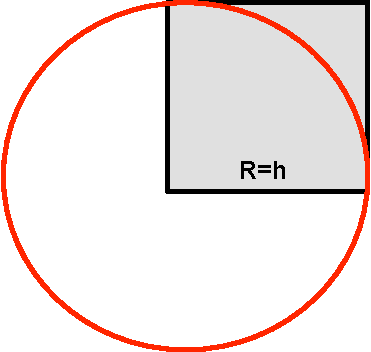
\includegraphics[width=4cm, height=4cm]{figures/source_size.pdf}
	\caption{Sketch showing the minimum source radius required according to mesh size to get a good solution approximation with the GFEM approach.}
	\label{fig:3.4}
\end{figure}

\clearpage
\subsection{Adding Refinement around the Source}
To be able to match the source size to that of the reference solution applying the GFEM  approach in a course mesh, I implement some local mesh refinement around the source location as shown in Figure \ref{fig:3.5}. Figures \ref{fig:3.6} and \ref{fig:3.7} show the seimograms for two GFEM cases in which local mesh refinement has been applied, exhibiting a good match with the reference solution. Figures \ref{fig:3.8} and \ref{fig:3.9} show the maximum cross correlation lag between GFEM solutions and the reference solution for each seismogram at 50 m from the source center, as well as two error types; one related to the maximum cross correlation ($E_{max}$) and the other one to the zero lag cross correlation ($E_0$). The lag fluctuates between -2 and 2 time steps for both GFEM cases. The observed maximum error corresponds to ($E_0$) and is around 3\%. These results show that these GFEM solutions with additional local mesh refinement around the source present an acceptable accuracy with respect to the reference solution.

% local mesh refinement around source
 \begin{figure}[h!]
	\centering
	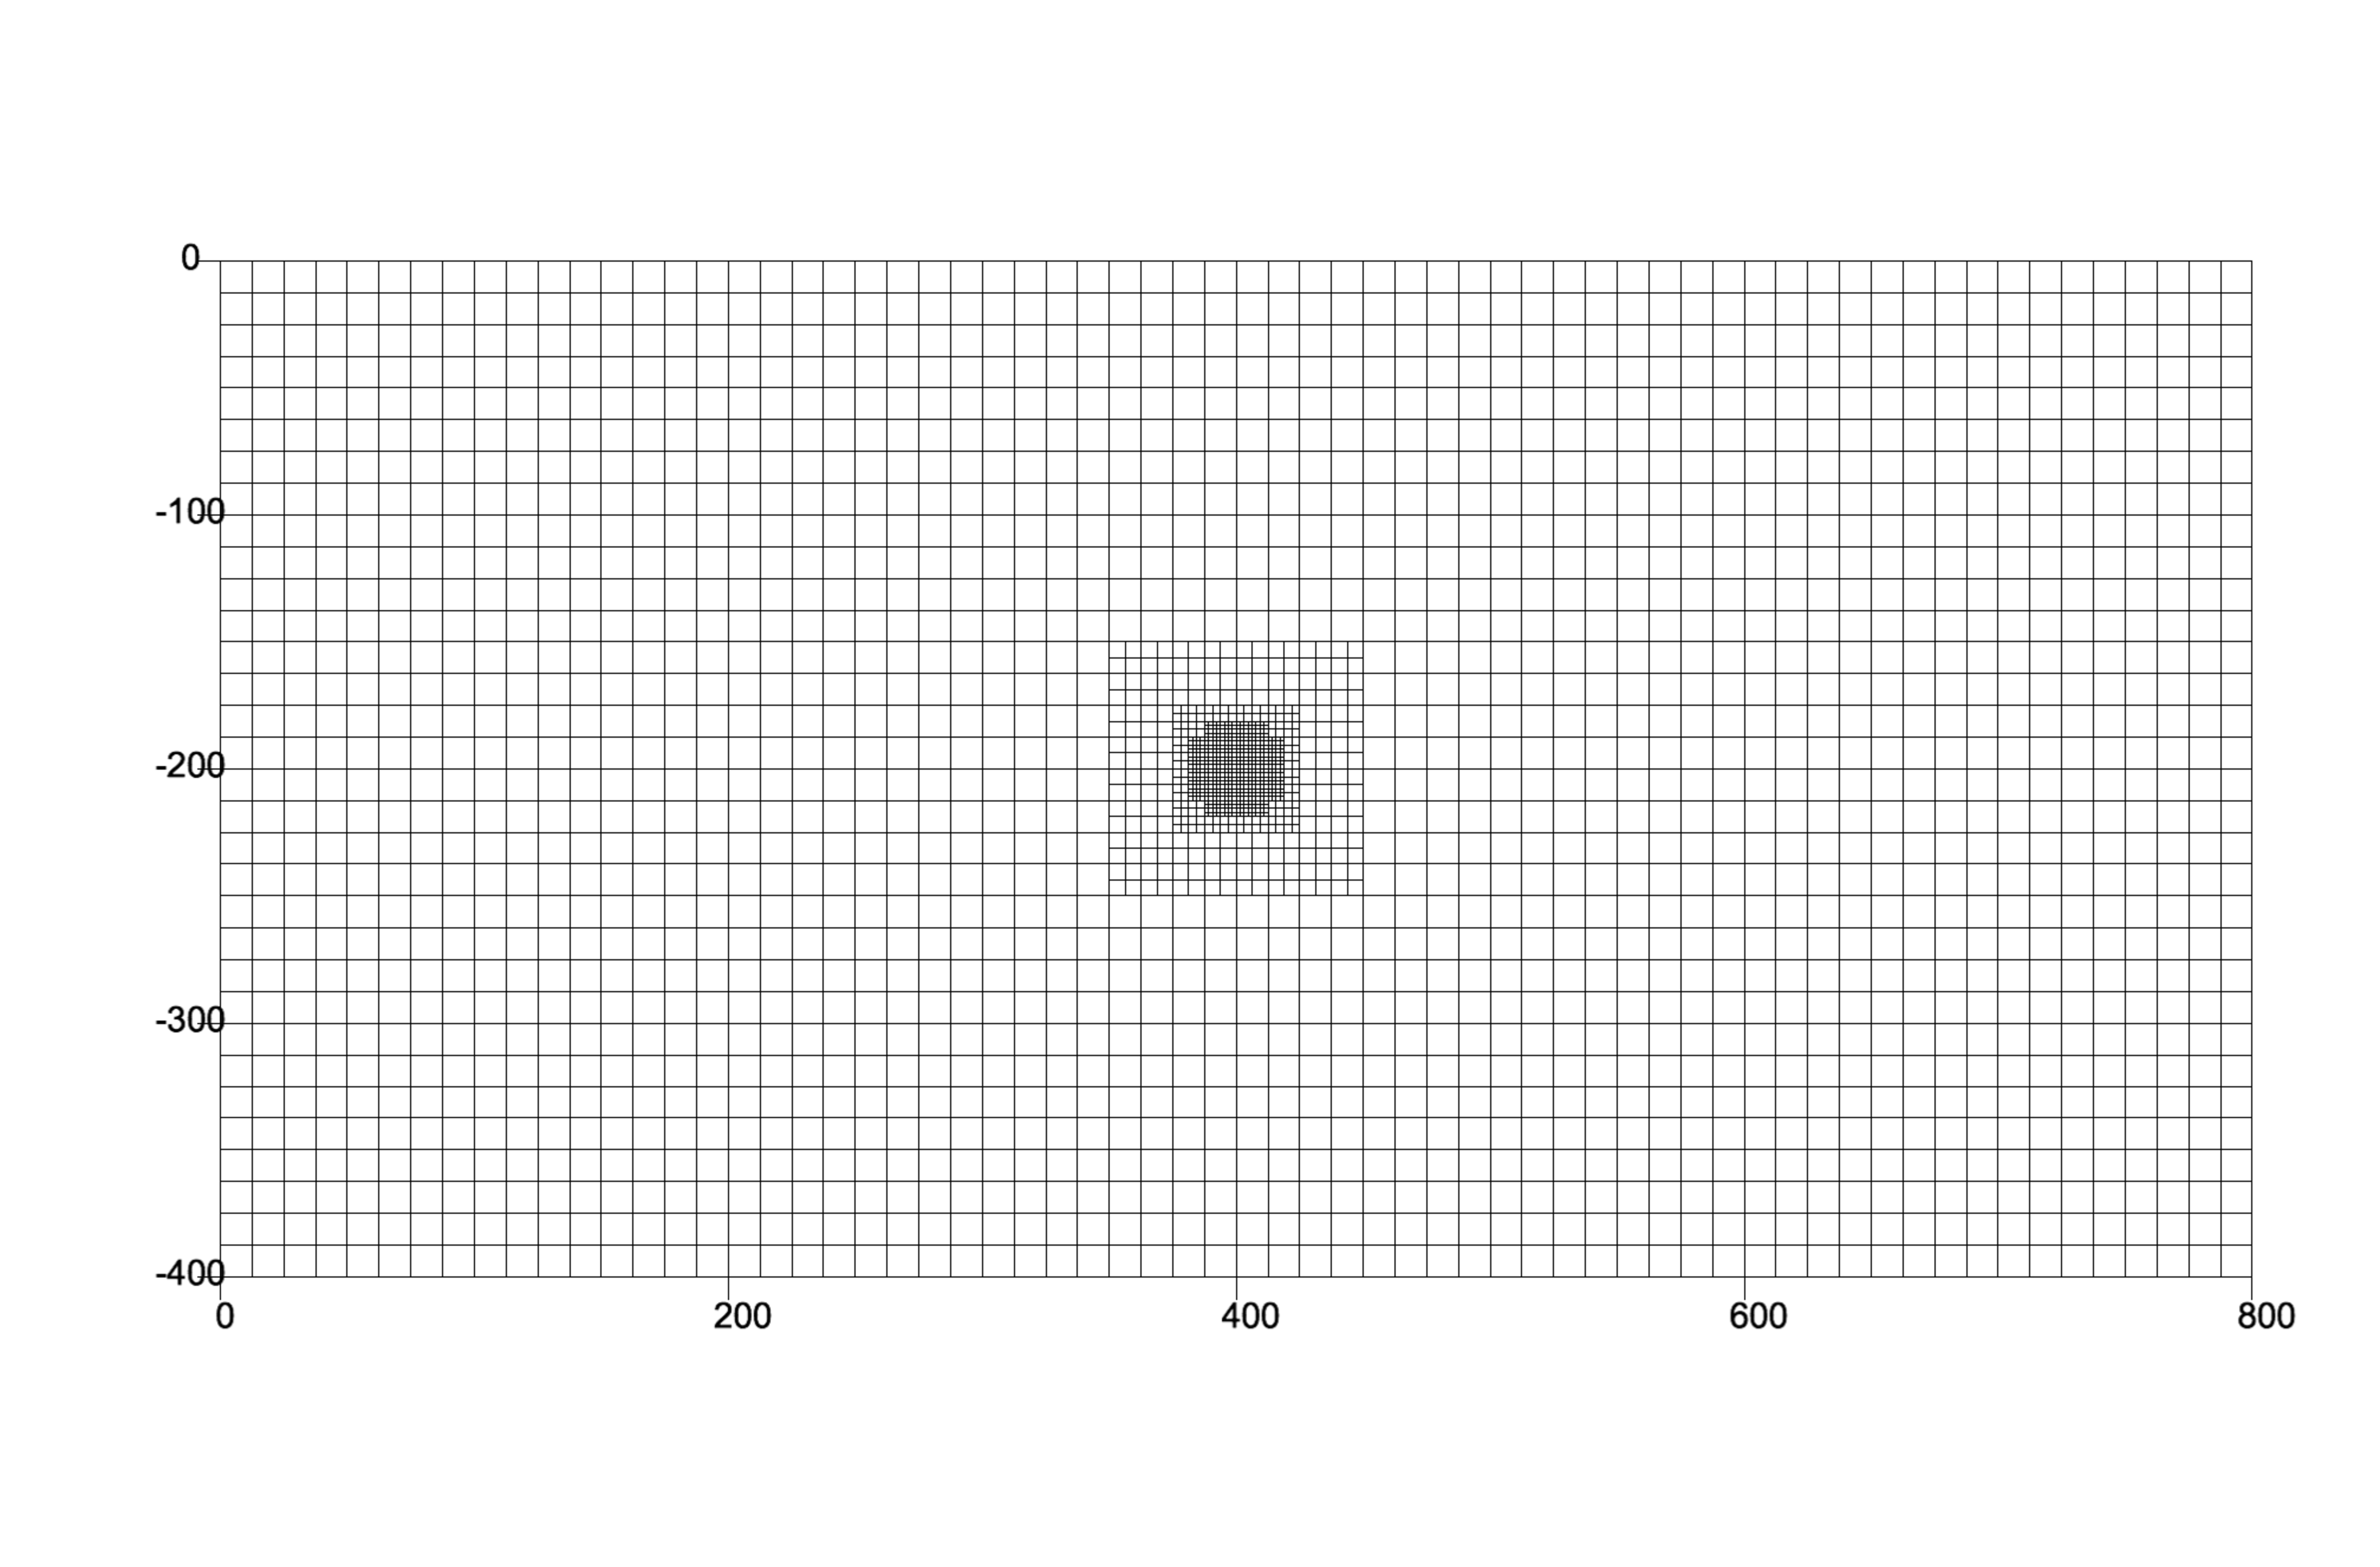
\includegraphics[width=14cm, height=7cm]{Thesis_Edith/figures/homo/h_source_doubleRef2.pdf}
	\caption{Coarse mesh with grid size of $8h$ used for GFEM simulations showing local mesh refinement around the source location.}
	\label{fig:3.5}
\end{figure}

% GFEM seismogram at 50 m from source
 \begin{figure}[h!]
 		\centering
		\begin{subfigure}{8cm}
				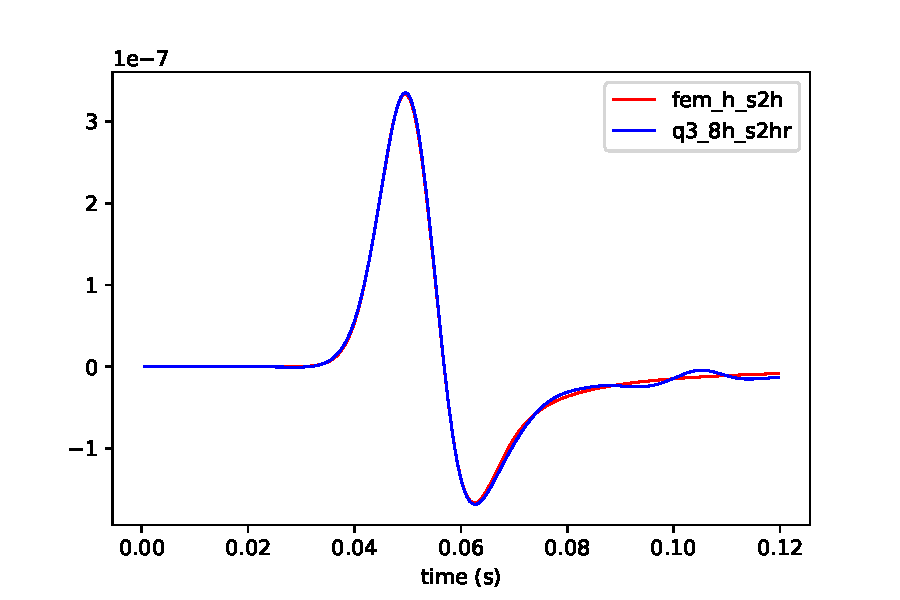
\includegraphics[width=8cm, height=6cm]{Thesis_Edith/figures/homo/homo_waves/fem_q3_8h_2hr_r50_0deg.pdf}
			     \caption{}
				%\label{fig:trace1}
		\end{subfigure}
        \hspace{0.25cm}
		\begin{subfigure}{8cm}
				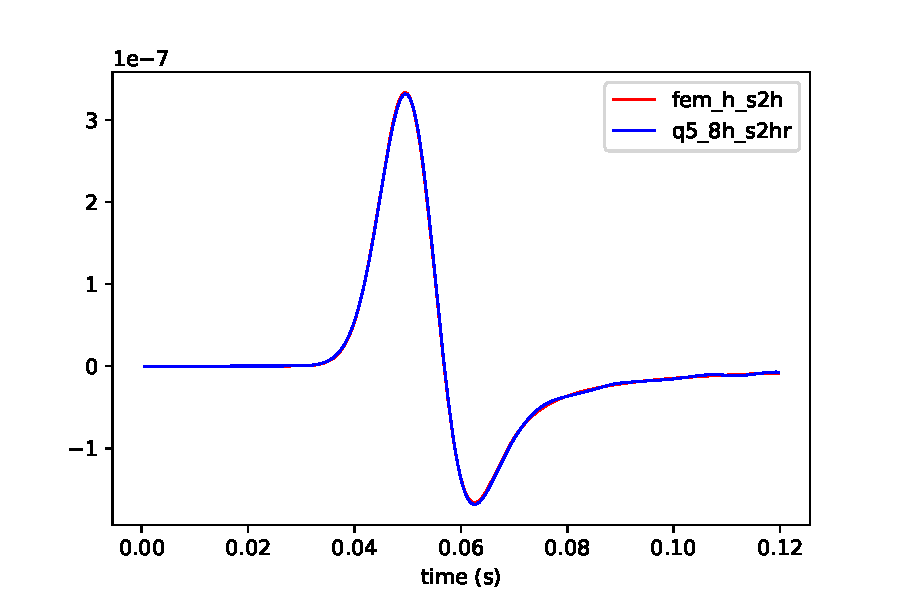
\includegraphics[width=8cm, height=6cm]{Thesis_Edith/figures/homo/homo_waves/fem_q5_8h_2hr_r50_0deg.pdf}
			   \caption{}
				%\label{fig:trace3}
		\end{subfigure}
 
	\caption{Homogeneous model: Seismograms for a receiver at 0 deg. and 50 m from the source center (see Figure \ref{fig:3.1}). GFEM solutions correspond to a mesh size of $8h$ and source radius of $2h$. (a) Seismograms for the reference solution and GFEM solution with plane waves in 3 directions. (b) Seismograms for the  reference solution and GFEM solution with plane waves in 5 directions.}  
	\label{fig:3.6}
\end{figure}

% GFEM seismogram at 100 m from source

 \begin{figure}[h!]
 		\centering
		\begin{subfigure}{8cm}
				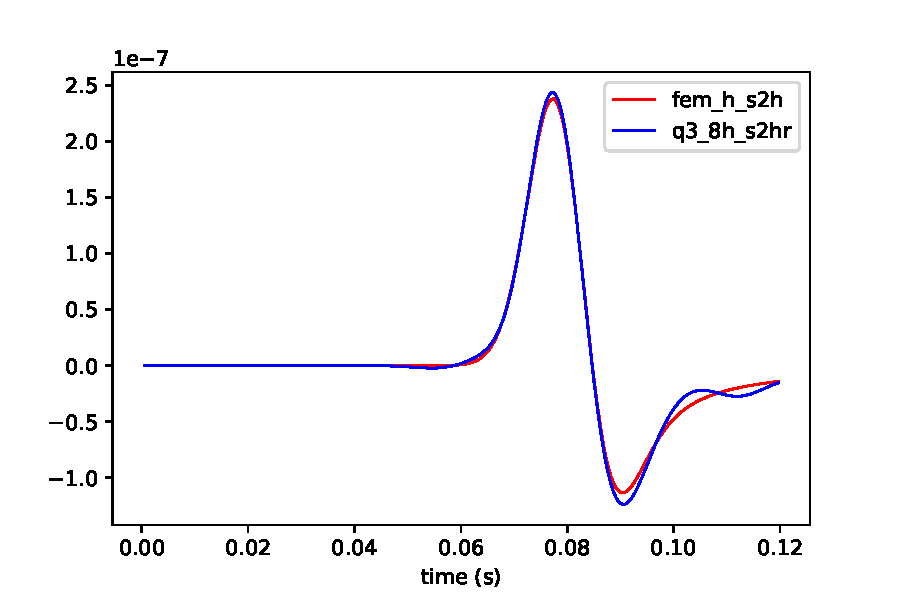
\includegraphics[width=8cm, height=6cm]{Thesis_Edith/figures/homo/homo_waves/fem_q3_8h_2hr_r100_0deg.pdf}
			     \caption{}
				%\label{fig:trace1}
		\end{subfigure}
        \hspace{0.25cm}
		\begin{subfigure}{8cm}
				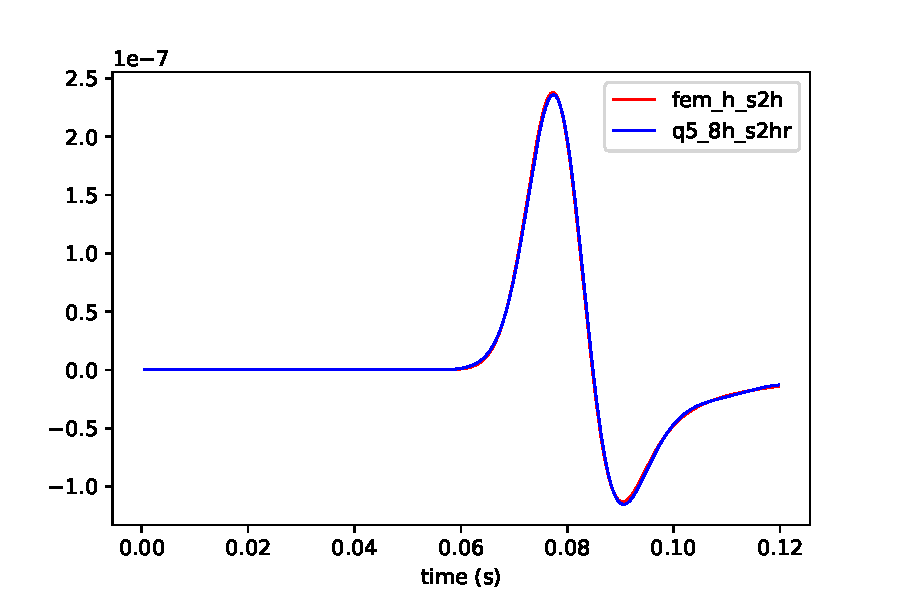
\includegraphics[width=8cm, height=6cm]{Thesis_Edith/figures/homo/homo_waves/fem_q5_8h_2hr_r100_0deg.pdf}
			   \caption{}
				%\label{fig:trace3}
		\end{subfigure}
 
	\caption{Homogeneous model: Seismograms for a receiver at 0 deg. and 100 m from the source center (see Figure \ref{fig:3.1}). GFEM solutions correspond to a mesh size of $8h$ and source radius of $2h$. (a) Seismograms for the reference solution and GFEM solution with plane waves in 3 directions. (b) Seismograms for the  reference solution and GFEM solution with plane waves in 5 directions.}  
	\label{fig:3.7}
\end{figure}

% GFEM Error @50m
 \begin{figure}[h!]
 		\centering
		\begin{subfigure}{8cm}
				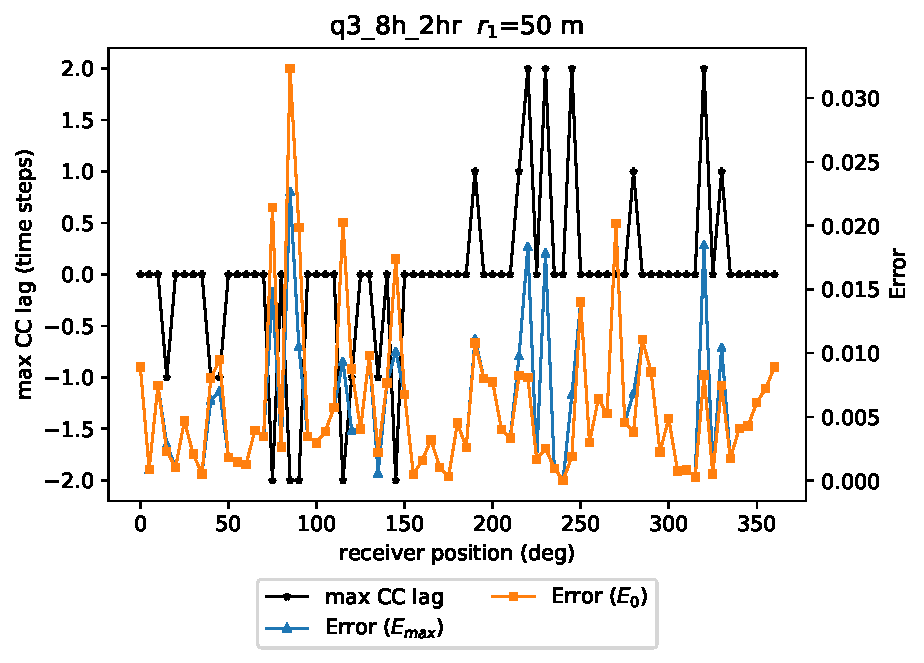
\includegraphics[width=8cm, height=6cm]{Thesis_Edith/figures/homo/homo_waves/Err_q3_8h_2hr_50m.pdf}
			     \caption{}
				%\label{fig:trace1}
		\end{subfigure}
        \hspace{0.25cm}
		\begin{subfigure}{8cm}
				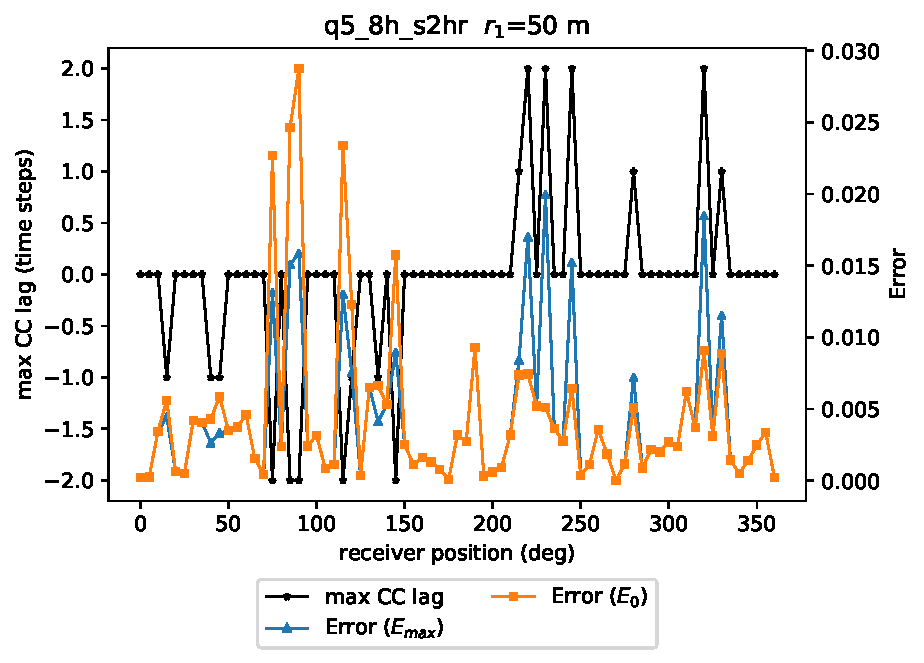
\includegraphics[width=8cm, height=6cm]{Thesis_Edith/figures/homo/homo_waves/Err_q5_8h_s2hr_50m.pdf}
			   \caption{}
				%\label{fig:trace3}
		\end{subfigure}
 
	\caption{Homogeneous model: Maximum cross correlation lag and errors for each receiver seismogram at 50 m from the source center for 2 GFEM cases with mesh size $8h$ and source size $2h$. (a) For the GFEM solution with 3 plane wave directions. (b) For the GFEM solution with 5 plane wave directions.}  
	\label{fig:3.8}
\end{figure}

% GFEM error @ 100 m
 \begin{figure}[h!]
 		\centering
		\begin{subfigure}{8cm}
				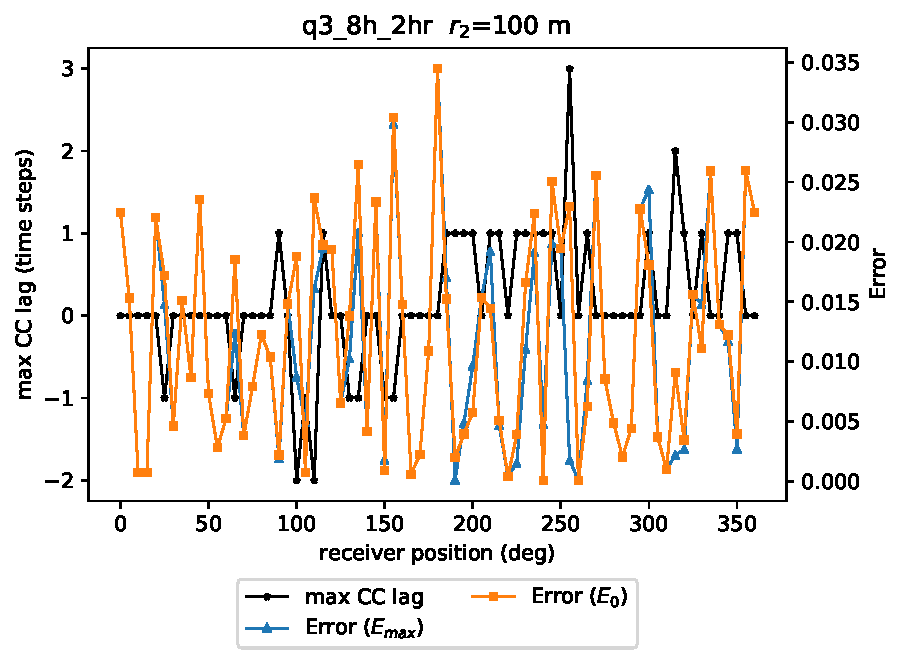
\includegraphics[width=8cm, height=6cm]{Thesis_Edith/figures/homo/homo_waves/Err_q3_8h_2hr_100m.pdf}
			     \caption{}
				%\label{fig:trace1}
		\end{subfigure}
        \hspace{0.25cm}
		\begin{subfigure}{8cm}
				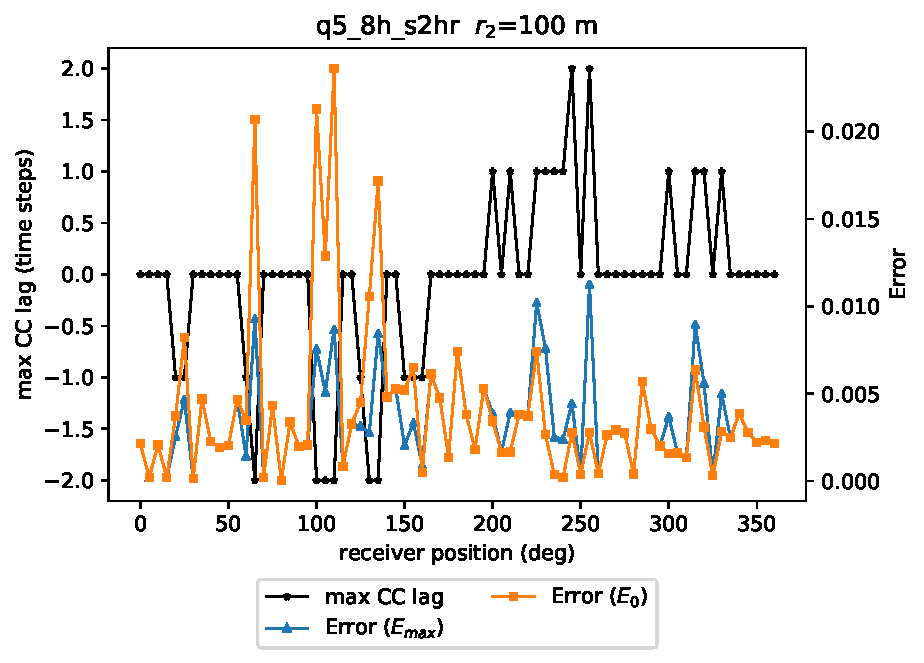
\includegraphics[width=8cm, height=5.5cm]{Thesis_Edith/figures/homo/homo_waves/Err_q5_8h_s2hr_100m.pdf}
			   \caption{}
				%\label{fig:trace3}
		\end{subfigure}
 
	\caption{Homogeneous model: Maximum cross correlation lag and errors for each receiver seismogram at 100 m from the source center for 2 GFEM cases with mesh size $8h$ and source size $2h$. (a) For the GFEM solution with 3 plane wave directions. (b) For the GFEM solution with 5 plane wave directions.}  
	\label{fig:3.9}
\end{figure}

\clearpage
\subsection{Performance Comparison}
To compare the accuracy and performance of GFEM solutions, I include two additional standard FEM solutions. Figure \ref{fig:3.10} shows the seismograms at 50 m and 100 m from the source center for two FEM solutions with coarser meshes than the reference solution. Figure \ref{fig:3.11} and \ref{fig:3.12} show the corresponding maximum cross correlation lag and errors. These results reveal that the solution accuracy deteriorates as the mesh size increases and in general the errors are greater than the GFEM cases with additional mesh refinement.

% fem seismograms
 \begin{figure}[h!]
 		\centering
		\begin{subfigure}{8cm}
				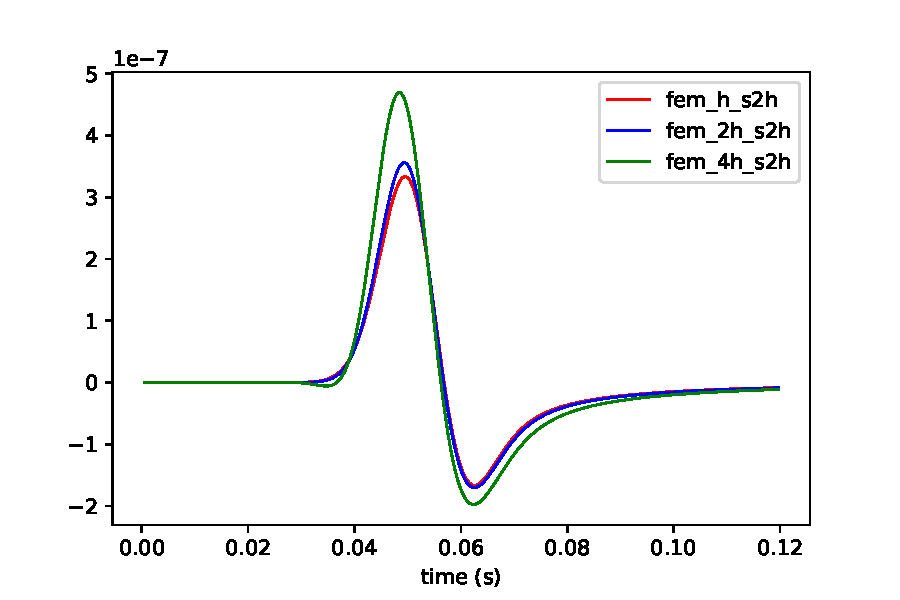
\includegraphics[width=8cm, height=6cm]{Thesis_Edith/figures/homo/homo_waves/fem_r50_0deg.pdf}
			     \caption{}
				%\label{fig:trace1}
		\end{subfigure}
        \hspace{0.25cm}
		\begin{subfigure}{8cm}
				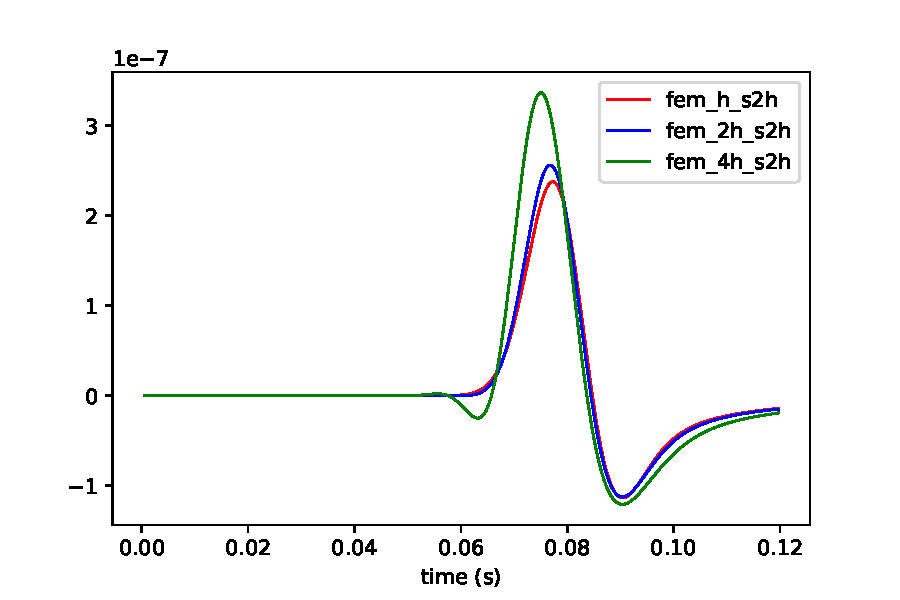
\includegraphics[width=8cm, height=6cm]{Thesis_Edith/figures/homo/homo_waves/fem_r100_0deg.pdf}
			   \caption{}
				%\label{fig:trace3}
		\end{subfigure}
 
	\caption{Homogeneous model: Seismograms for the reference solution and two additional FEM solutions with mesh size $2h$ and $4h$. (a) Seismograms at 0 deg and 50 m from the source center. (b) Seismograms at 0 deg and 100 m from the source center.}  
	\label{fig:3.10}
\end{figure}

% fem errorrs
 \begin{figure}[h!]
 		\centering
		\begin{subfigure}{8cm}
				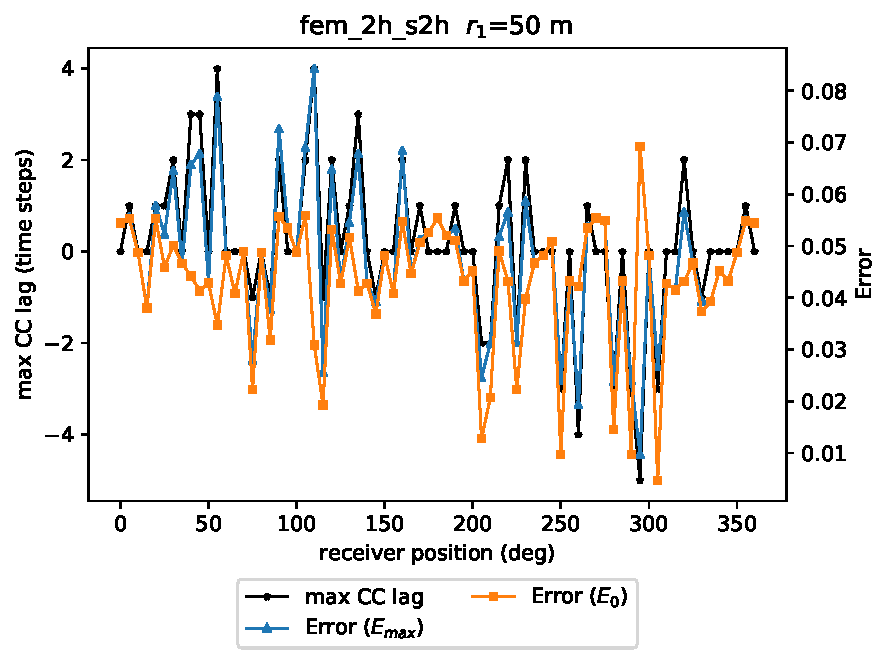
\includegraphics[width=8cm, height=6cm]{Thesis_Edith/figures/homo/homo_waves/Err_fem_2h_s2h_50m.pdf}
			     \caption{}
				%\label{fig:trace1}
		\end{subfigure}
        \hspace{0.25cm}
		\begin{subfigure}{8cm}
				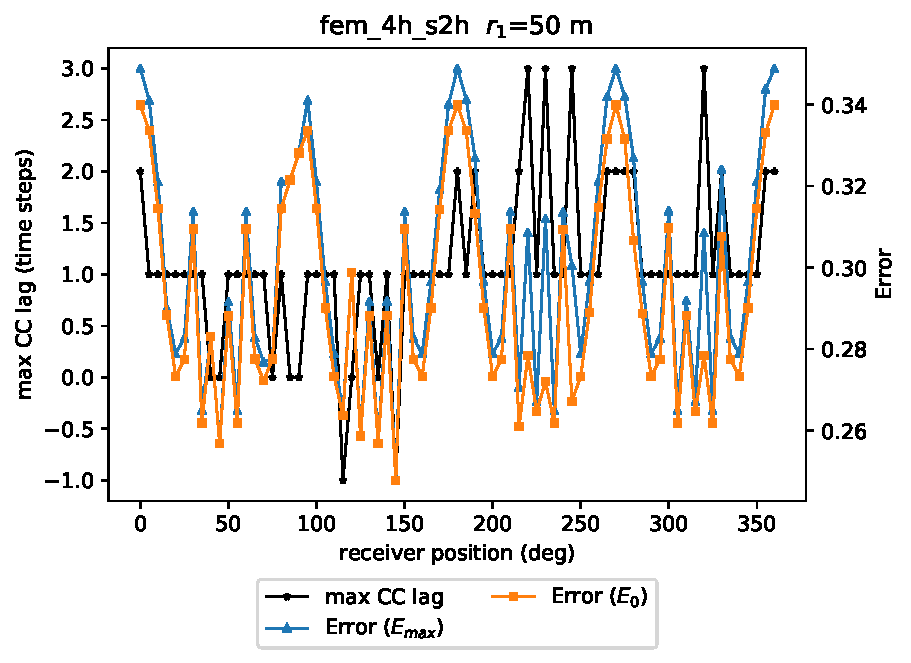
\includegraphics[width=8cm, height=6cm]{Thesis_Edith/figures/homo/homo_waves/Err_fem_4h_s2h_50m.pdf}
			   \caption{}
				%\label{fig:trace3}
		\end{subfigure}
 
	\caption{Homogeneous model: Maximum cross correlation lag and errors for seismograms for each receiver at 50 m from the source center for 2 FEM cases. (a) For the FEM solution with mesh size of $2h$. (b) For the FEM solution with mesh size of $4h$.}  
	\label{fig:3.11}
\end{figure}

 \begin{figure}[h!]
 		\centering
		\begin{subfigure}{8cm}
				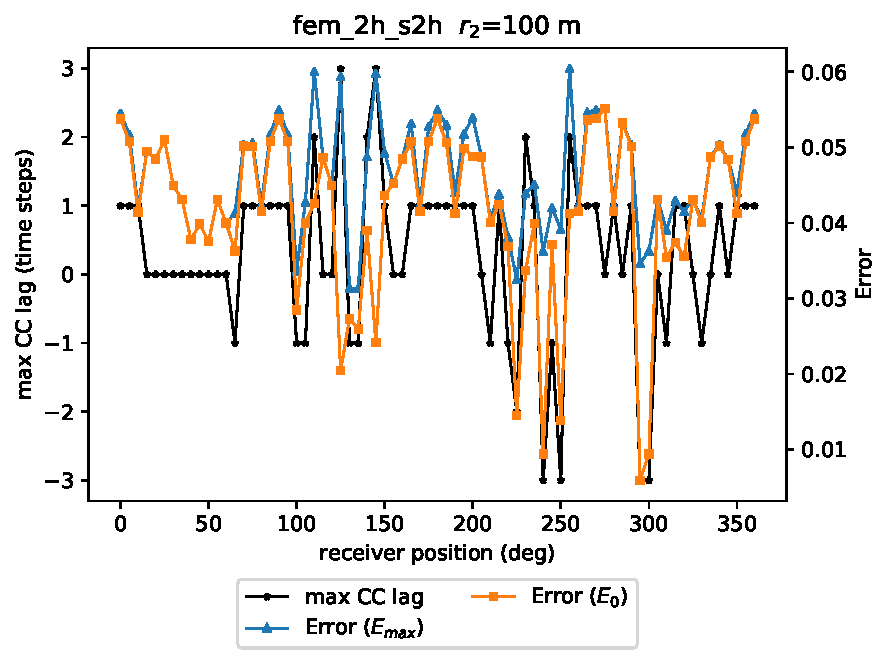
\includegraphics[width=8cm, height=6cm]{Thesis_Edith/figures/homo/homo_waves/Err_fem_2h_s2h_100m.pdf}
			     \caption{}
				%\label{fig:trace1}
		\end{subfigure}
        \hspace{0.25cm}
		\begin{subfigure}{8cm}
				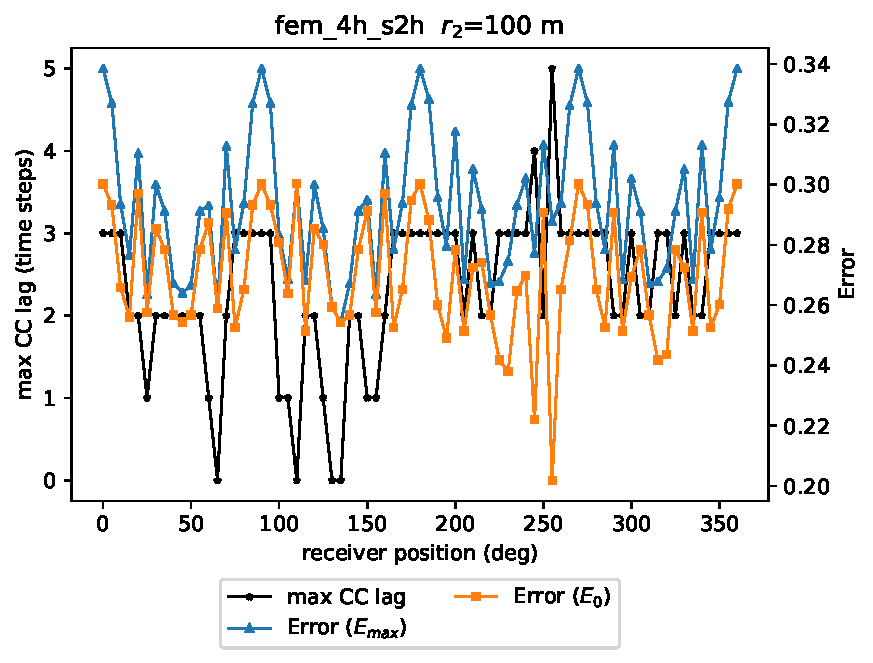
\includegraphics[width=8cm, height=6cm]{Thesis_Edith/figures/homo/homo_waves/Err_fem_4h_s2h_100m.pdf}
			   \caption{}
				%\label{fig:trace3}
		\end{subfigure}
 
	\caption{Homogeneous model: Maximum cross correlation lag and errors for seismograms for each receiver at 100 m from the source center for 2 FEM cases (a) For the FEM solution with mesh size of $2h$. (b) For the FEM solution with mesh size of $4h$.}  
	\label{fig:3.12}
\end{figure}

Figure \ref{fig:3.13} shows the the mean error versus relative simulation time and standard deviation for the additional standard FEM solutions and for various GFEM cases. the  GFEM cases correspond to  solutions with a coarse mesh  of $8h$ and with a source radius of $8h$ and $2h$. An additional GFEM result with mesh and source radius size of $4h$ is also presented. The relative simulation time were calculated as a ratio taken with respect to the reference FEM solution and the mean error is the mean of all seismogram errors at 50 and 100 m from the center of the source. For all the GFEM results, except for the case of mesh size $4h$ and plane waves in 3 directions (q3\_4h\_4h), the mean error is lower than any of the two additional FEM cases. Among The GFEM cases, the examples with the additional mesh refinement exhibit the least error and standard deviation. The GFEM solutions also present a faster simulation time than the reference solution, it is around 0.2 times the reference solution. 

% Mean error
 \begin{figure}[h!]

		\begin{subfigure}{8cm}
				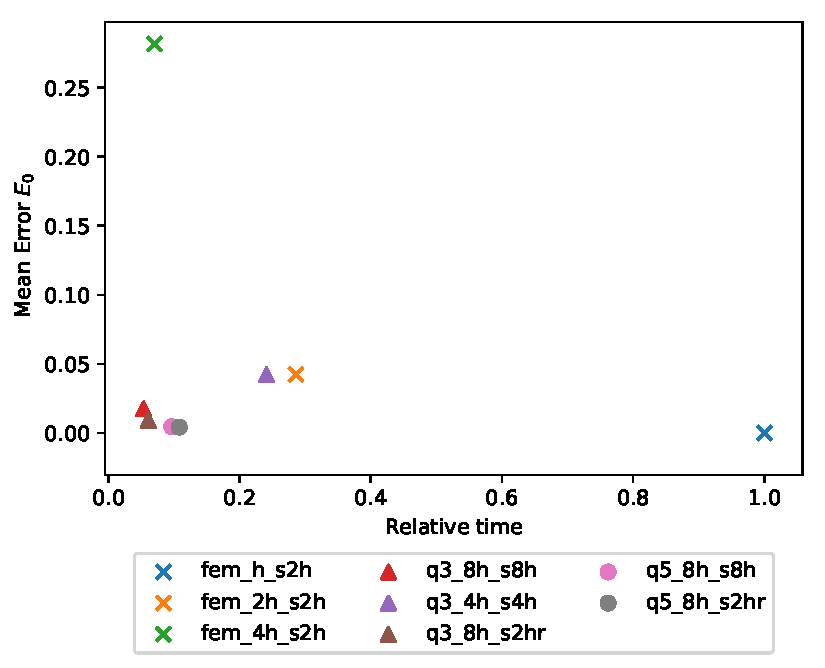
\includegraphics[width=8cm, height=6cm]{Thesis_Edith/figures/homo/homo_waves/MeanError_time_radial.pdf}
			   \caption{}
				%\label{fig:3.7b}
	    \hspace{0.25cm}	
		\end{subfigure}
				\begin{subfigure}{8cm}
				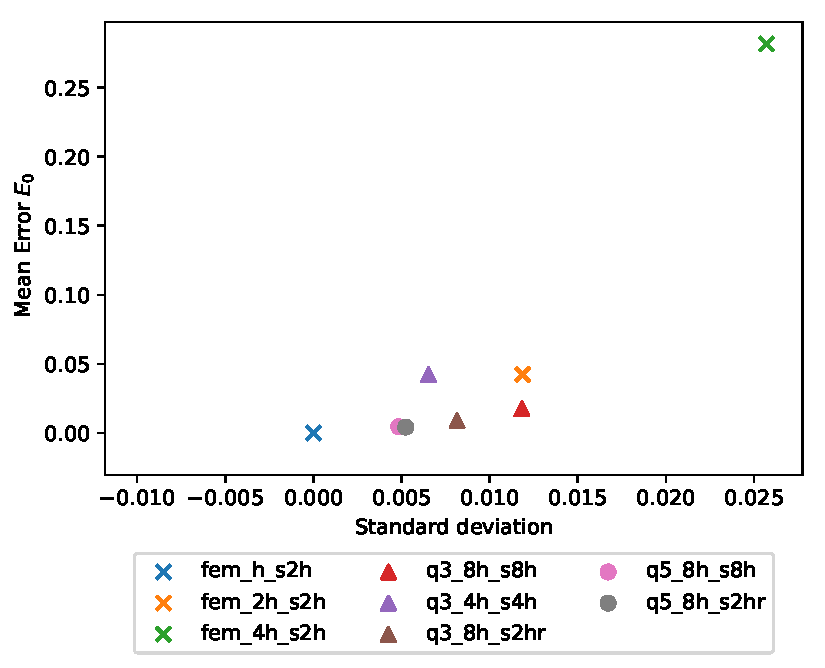
\includegraphics[width=8cm, height=6.3cm]{Thesis_Edith/figures/homo/homo_waves/Error_std_radial.pdf}
				\caption{}
				%\label{fig:3.7b}
		\end{subfigure}
 
	\caption{Homogeneous model: Mean error vs relative time and standard deviation for various FEM and GFEM cases. (a) Mean error vs relative time. (b) Mean error vs standard deviation}
	\label{fig:3.13}
\end{figure}

% New section: Layered Model
\section{Case 2: Layered Medium with Low Velocity Layer}
 The model for this example is as shown in Figure \ref{fig:3.14}, where $h_i$  and $v_i$ are the thickness and acoustic velocity of $i-th$ layer respectively. Notice that in this case the top layer presents a relative low velocity respect to the other two.  The source is located at a depth of - 50m and and at 400 m in the horizontal coordinate. There are also 50 receivers spanning from 400 m, directly above from the source, to 750 m in the horizontal coordinate very close to surface. For this case, I also find a FEM reference solution in a fine mesh of size $h$ with source radius of $2h$. I find as well 2 additional FEM solutions in mesh sizes of $2h$ and $4h$. I also obtain GFEM solutions in a coarse mesh of $8h$ and source sizes of  $8h$ and $2h$.  For all the GFEM cases the wave number used for the plane wave enrichments is 0.14 m$^{-1}$, calculated by dividing the source radial frequency by the lowest velocity (1800 m/s).
 
 Table \ref{table:3.1} shows the wavelength and wavenumber for the different layers according to their velocity. It also shows the number of cells per wavelength for the different meshes used.   
 Figure \ref{fig:3.15} shows the seismograms for the reference solution for the shot gather configuration of Figure \ref{fig:3.14}.
 
 \begin{figure}[h!]
	\centering
	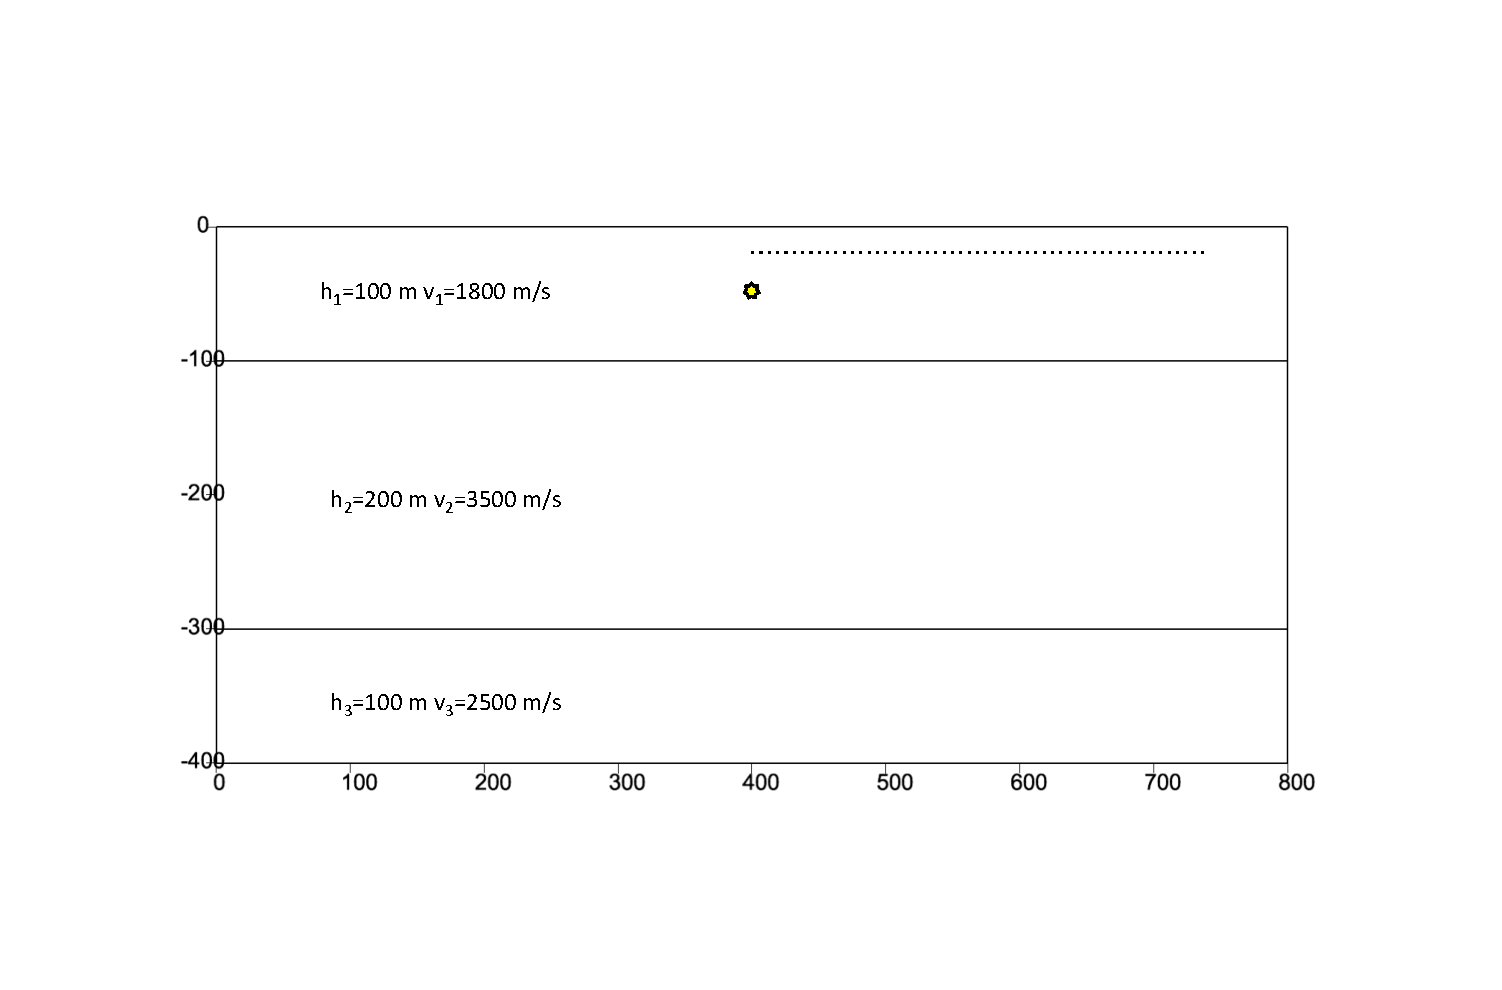
\includegraphics[width=14cm, height=7cm]{Thesis_Edith/figures/layered_model/layer_source.pdf}
	\caption{Three-layer model  with a seismic source in the first layer (yellow star) and a horizontal array of 50 receivers close to surface as depicted by the dotted line.}
	\label{fig:3.14}
\end{figure}

%table
\begin{table}[h!]
\footnotesize
\centering
    \begin{tabular}{|c|m{2cm}|m{2cm}|m{2cm}| m{1cm}|m{1cm}|m{1cm}|m{1cm}|}
      \hline
      \multirow{2}{*}{Layer} &
      \multirow{2}{2cm}{Velocity (m/s)} &
      \multirow{2}{2cm}{Wavelength \quad $\lambda$ (m)} &
      \multirow{2}{2cm}{Wavenumber  k (m$^{-1}$)} &
         \multicolumn{4}{m{4cm}|}{Number cells per wavelength in a mesh size of:} \\
         & & & & $h$ & $2h$ & $4h$ & $8h$ \\
      \hline
      1 & 1800 & 45 & 0.14 & 28.8 & 14.4 & 7.2 & 3.6\\
      \hline
      2 & 3500 & 87.5 & 0.07 & 56 & 28 & 14 & 7\\
      \hline
      3 & 2500 & 62.5 & 0.10 & 40 & 20 & 10 & 5\\
      \hline
    \end{tabular}
    \caption{Layered model: Table showing the velocity, wavelength and wavenumber for each layer, as well as the number of cells per wavelength in different mesh sizes. Source frequency is 40 Hz and $h=$1.5625 m}
    \label{table:3.1}
\end{table}

%shot gather
 \begin{figure}[h!]
	\centering
	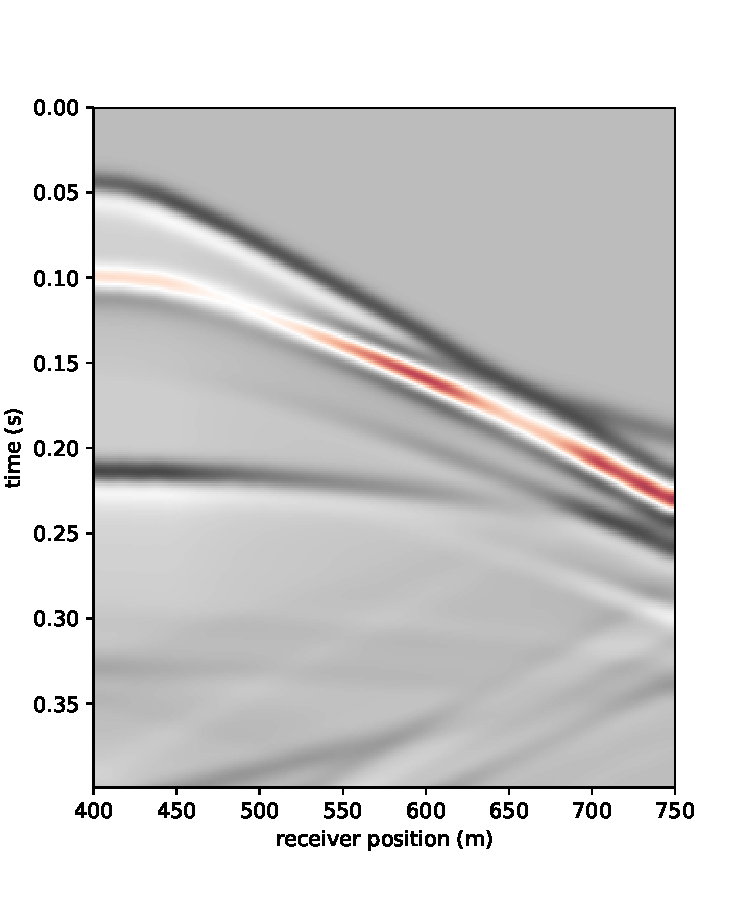
\includegraphics[width=10cm, height=13cm]{Thesis_Edith/figures/layered_model/layer_waves/seismogram_layered.pdf}
	\caption{Layered model: Seismograms of the shot gather as depicted in Figure \ref{fig:3.14} of the reference solution. Coefficient for the divergence correction is 2.5.}
	\label{fig:3.15}
\end{figure}

%************
\clearpage
Figure \ref{fig:3.16} presents the seismograms for different FEM solutions, including the reference one, for receivers located at 400 m and 750 m in the horizontal coordinate. (See Figure \ref{fig:3.14}). These results show that FEM solutions degrade as the mesh gets coarser and as the receiver gets further away from the source location.
Figures \ref{fig:3.17} and  \ref{fig:3.18} present GFEM solutions with 3 and 5 plane wave directions and for source radii of $8h$ ( Figure \ref{fig:3.17})  and $2h$ (Figure \ref{fig:3.18}). In general, the solution improves as the number of plane waves used increases and the source size decreases. However the GFEM solutions with 3 plane waves directions present some ringing in the waveforms. This observation suggests that 3 plane wave directions is too few to obtain a stable solution with this mesh size.

% Traces
%*******
 \begin{figure}[h!]
 		\centering
		\begin{subfigure}{8cm}
				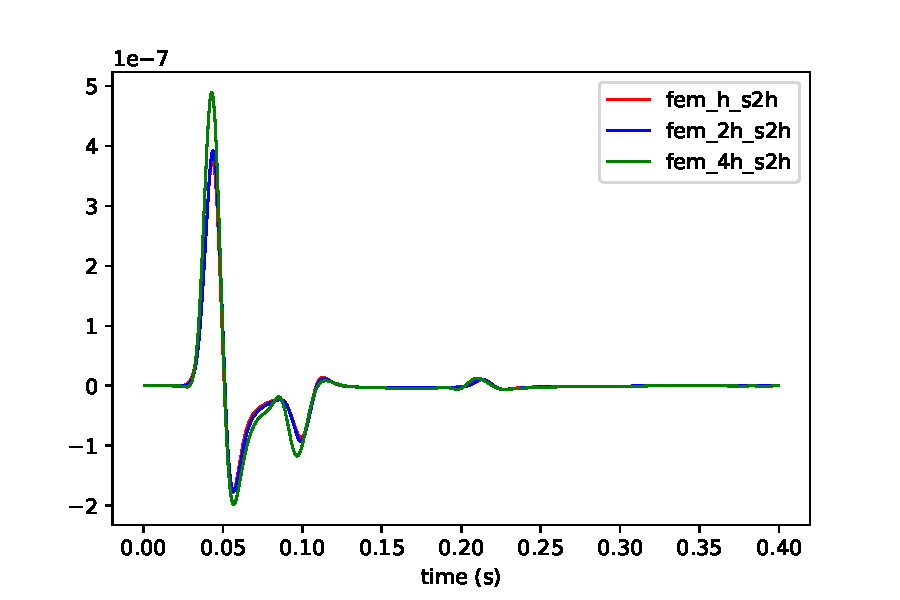
\includegraphics[width=8cm, height=5.5cm]{Thesis_Edith/figures/layered_model/layer_waves/fem_layered_tr1.pdf} 
			     \caption{}
				%\label{fig:3.7a}
		\end{subfigure}
        \hspace{0.25cm}	
		\begin{subfigure}{8cm}
				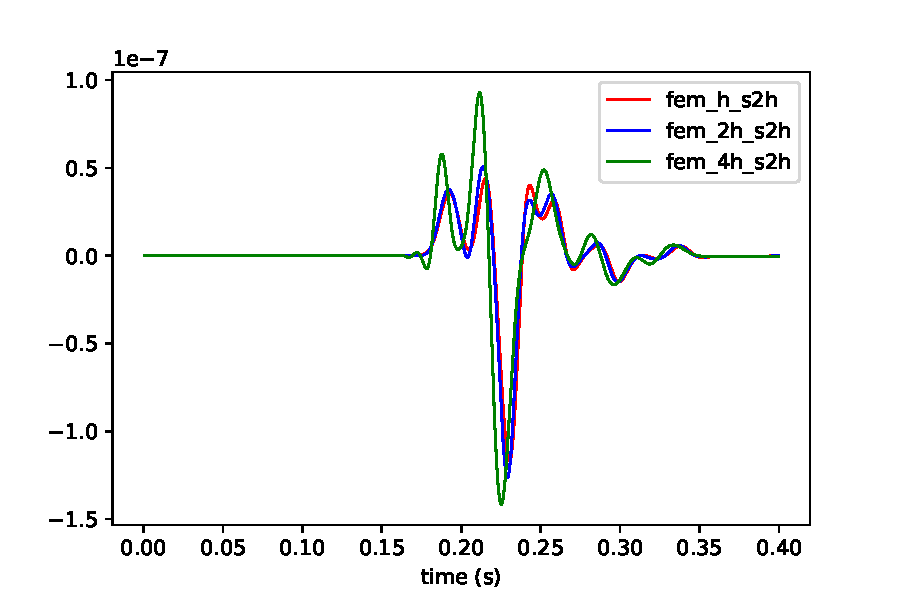
\includegraphics[width=8cm, height=5.5cm]{Thesis_Edith/figures/layered_model/layer_waves/fem_layered_tr50.pdf}
			   \caption{}
				%\label{fig:3.7b}
		\end{subfigure}
 
	\caption{Layered model: Seimograms of the reference solution and 2 additional FEM solutions in coarser meshes. (a) Seimograms from a receiver placed at 400 m in the layered model. (b) Seimograms from a receiver placed at 750 m in the layered model.}
	\label{fig:3.16}
\end{figure}

%GFEM traces
 \begin{figure}[h!]
 		\centering
		\begin{subfigure}{8cm}
				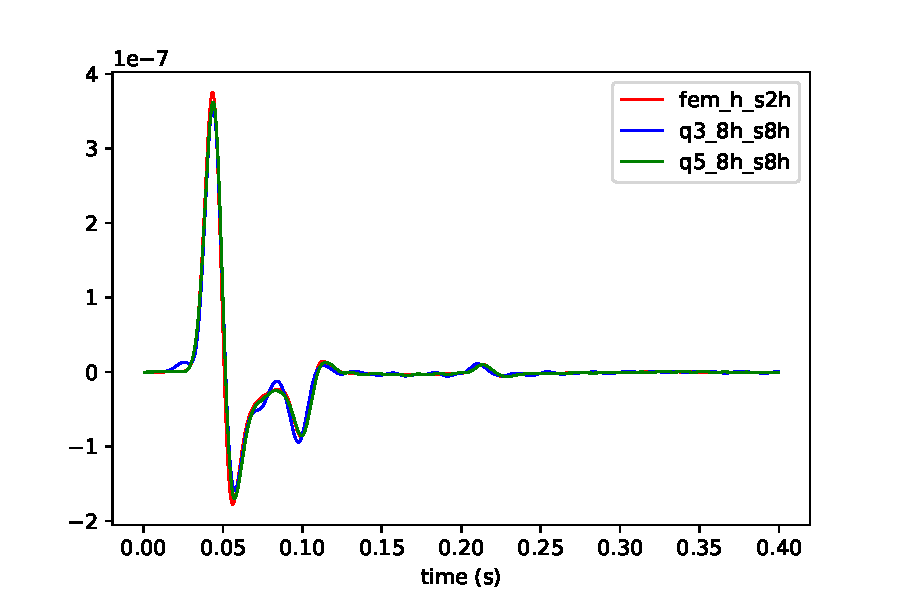
\includegraphics[width=8cm, height=5.5cm]{Thesis_Edith/figures/layered_model/layer_waves/gfem_layered_tr1.pdf} 
			     \caption{}
				%\label{fig:3.7a}
		\end{subfigure}
        \hspace{0.25cm}	
		\begin{subfigure}{8cm}
				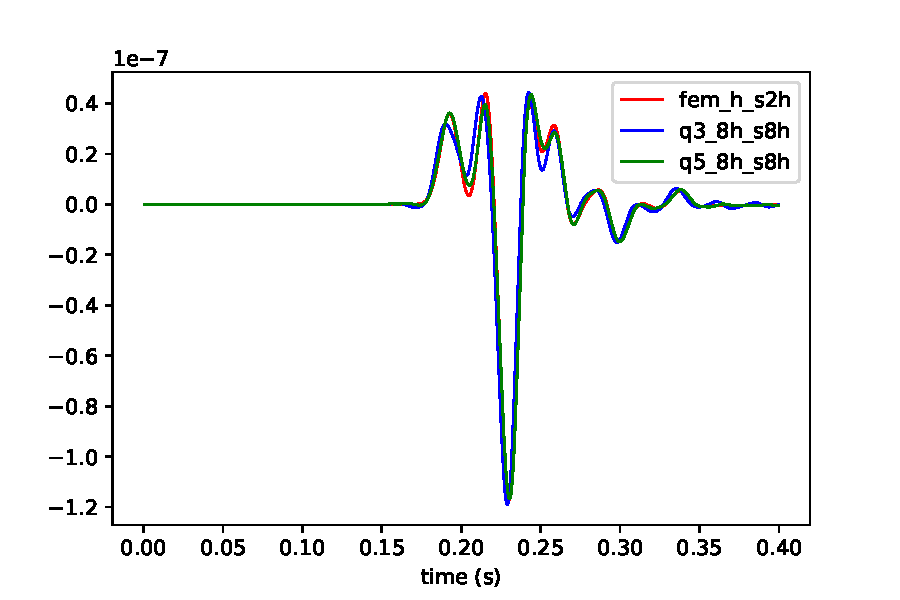
\includegraphics[width=8cm, height=5.5cm]{Thesis_Edith/figures/layered_model/layer_waves/gfem_layered_tr50.pdf}
			   \caption{}
				%\label{fig:3.7b}
		\end{subfigure}
 
	\caption{Layered model: Seismograms of the reference solution and 2 GFEM solutions with 3 and 5 plane wave directions, using a mesh and source size of $8h$. (a) Seimograms from a receiver placed at 400 m in the layered model. (b) Seimograms from a receiver placed at 750 m in the layered model.}
	\label{fig:3.17}
\end{figure}

%GFEMh traces
 \begin{figure}[h!]
 		\centering
		\begin{subfigure}{8cm}
				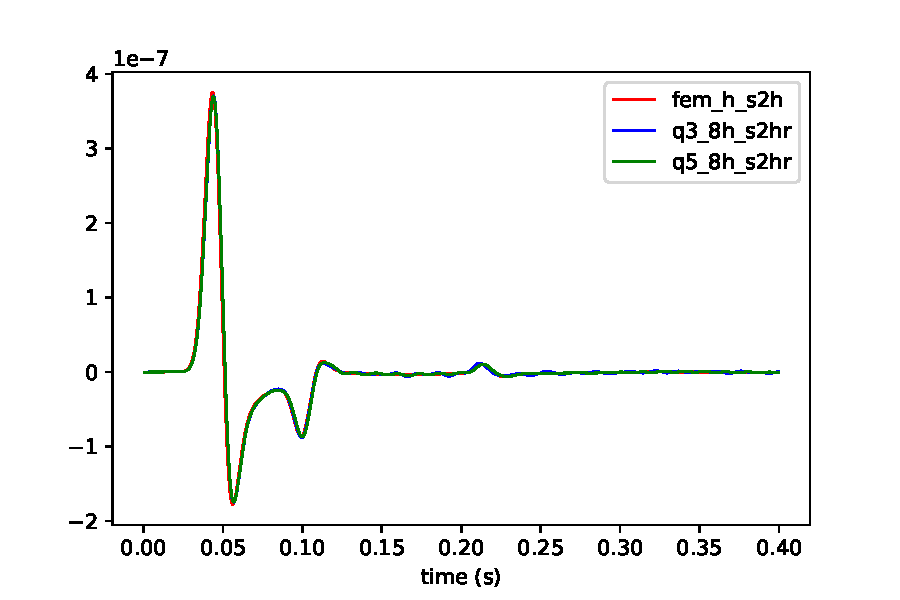
\includegraphics[width=8cm, height=5.5cm]{Thesis_Edith/figures/layered_model/layer_waves/gfemh_layered_tr1.pdf} 
			     \caption{}
				%\label{fig:3.7a}
		\end{subfigure}
        \hspace{0.25cm}	
		\begin{subfigure}{8cm}
				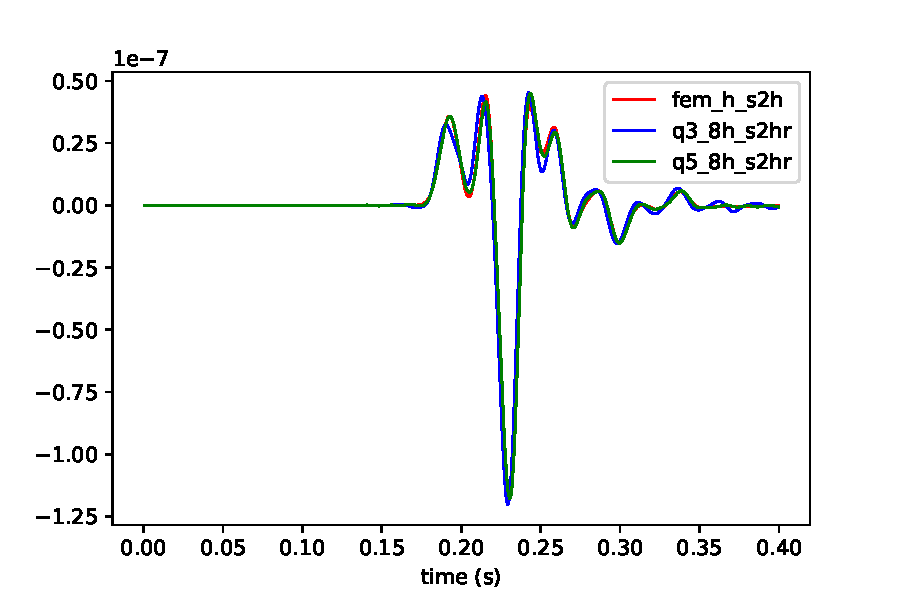
\includegraphics[width=8cm, height=5.5cm]{Thesis_Edith/figures/layered_model/layer_waves/gfemh_layered_tr50.pdf}
			   \caption{}
				%\label{fig:3.7b}
		\end{subfigure}
 
	\caption{Layered model: Seismograms of the reference solution and 2 GFEM solutions with 3 and 5 plane wave directions, using a mesh size of $8h$ and source size of $2h$. (a) Seimograms from a receiver placed at 400 m in the layered model. (b) Seimograms from a receiver placed at 750 m in the layered model.}
	\label{fig:3.18}
\end{figure}

%****
\clearpage
 Figure \ref{fig:3.19} presents the maximum cross correlation lag and two error types with respect to the reference solution for the two FEM cases calculated at the 50 receiver seismograms . Notice that the maximum cross correlation lag tend to increase as the receiver position gets further away from the source center. This effect is stronger for the FEM case with the coarsest mesh ($4h$). The errors corresponding for this FEM case are also the greatest. In general the error related to the maximum cross correlation ($E_{max}$)  is lower than the error related to the zero cross correlation $E_0$, showing the effect of mesh dispersion in the results.
 
 Figures \ref{fig:3.20} and \ref{fig:3.21} present the maximum cross correlation lag and two types of error for various GFEM cases for the 50 receiver seismograms. Figure \ref{fig:3.20} shows the effect of source size for GFEM solutions with 3 plane waves directions and Figure \ref{fig:3.21} does it for the GFEM solution with 5 plane waves directions. These results reveal that the errors decrease for  GFEM solutions when compared to the 2 FEM cases in  Figure \ref{fig:3.19} and that decreasing source radius further decreases the errors. Notice that, specially for the GFEM case with 5 plane wave directions, the lag and error are consistent across the 50 receivers, revealing less dispersive effects despite of using a very coarse mesh.
 
%Fem error
 \begin{figure}[h!]
 		\centering
		\begin{subfigure}{8cm}
				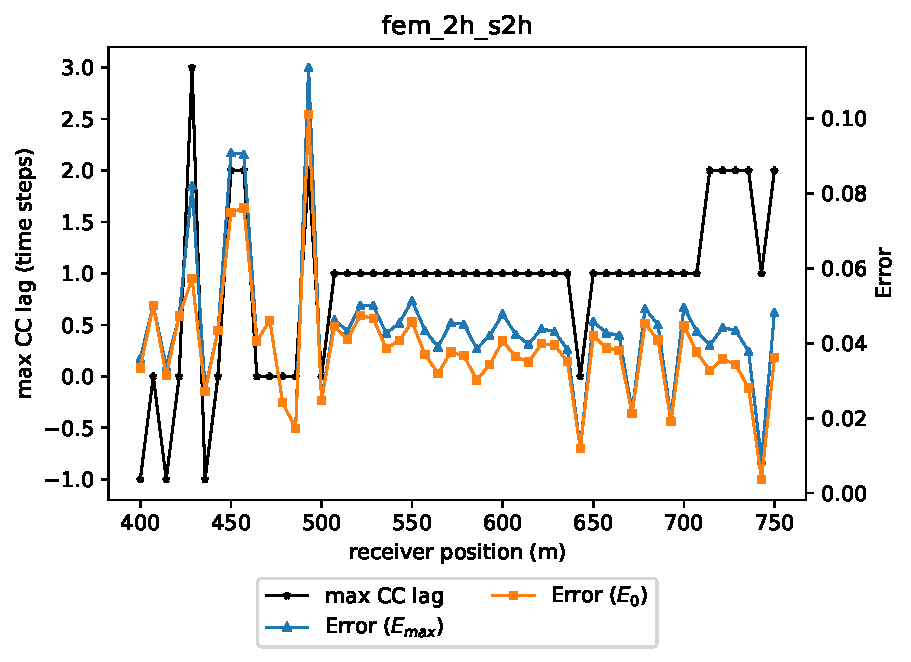
\includegraphics[width=8cm, height=5.5cm]{Thesis_Edith/figures/layered_model/layer_waves/Err_fem_2h_s2h.pdf}
			     \caption{}
				%\label{fig:3.7a}
		\end{subfigure}
        \hspace{0.25cm}	
		\begin{subfigure}{8cm}
				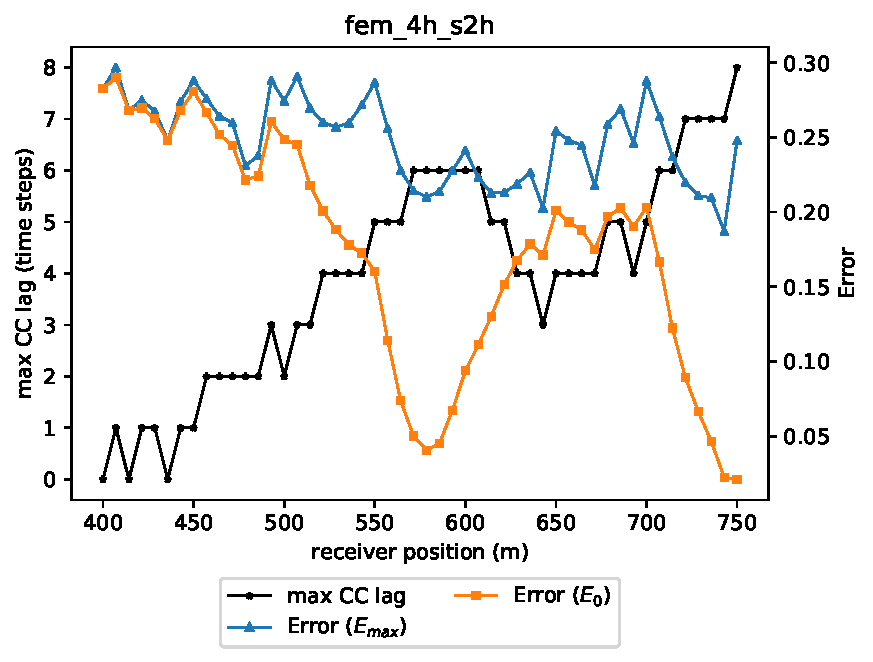
\includegraphics[width=8cm, height=5.5cm]{Thesis_Edith/figures/layered_model/layer_waves/Err_fem_4h_s2h.pdf}
			   \caption{}
				%\label{fig:3.7b}
		\end{subfigure}
 
	\caption{Layered model: Maximum cross correlation lag and errors for each receiver seismogram for 2 FEM cases. (a) For the FEM solution with mesh size of $2h$.(b) For the FEM solution with mesh size of $4h$.}
	\label{fig:3.19}
\end{figure}

%gFem error
 \begin{figure}[h!]
 		\centering
		\begin{subfigure}{8cm}
				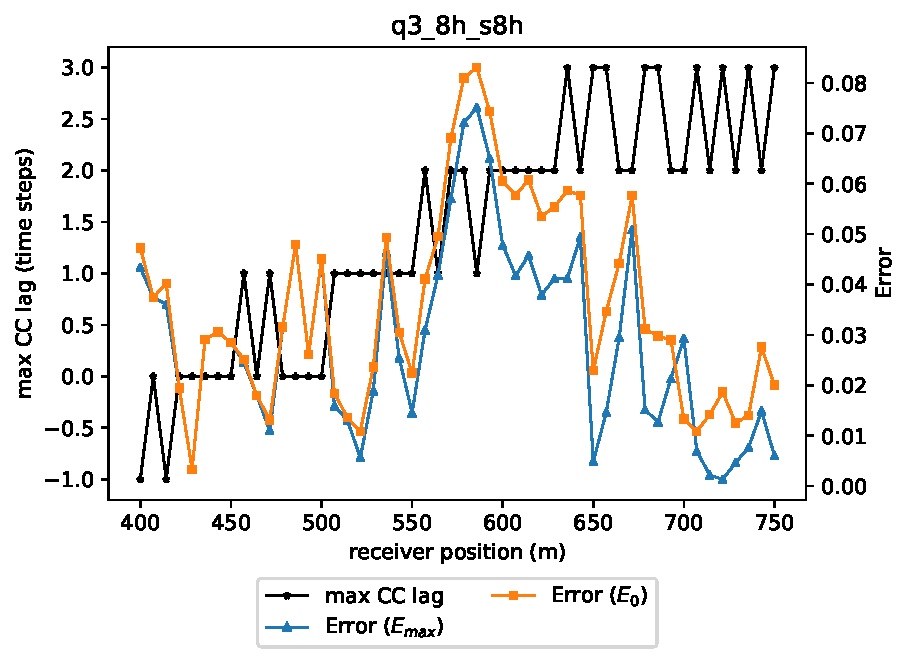
\includegraphics[width=8cm, height=6cm]{Thesis_Edith/figures/layered_model/layer_waves/Err_q3_8h_s8h.pdf}
			     \caption{}
				%\label{fig:3.7a}
		\end{subfigure}
        \hspace{0.25cm}	
		\begin{subfigure}{8cm}
				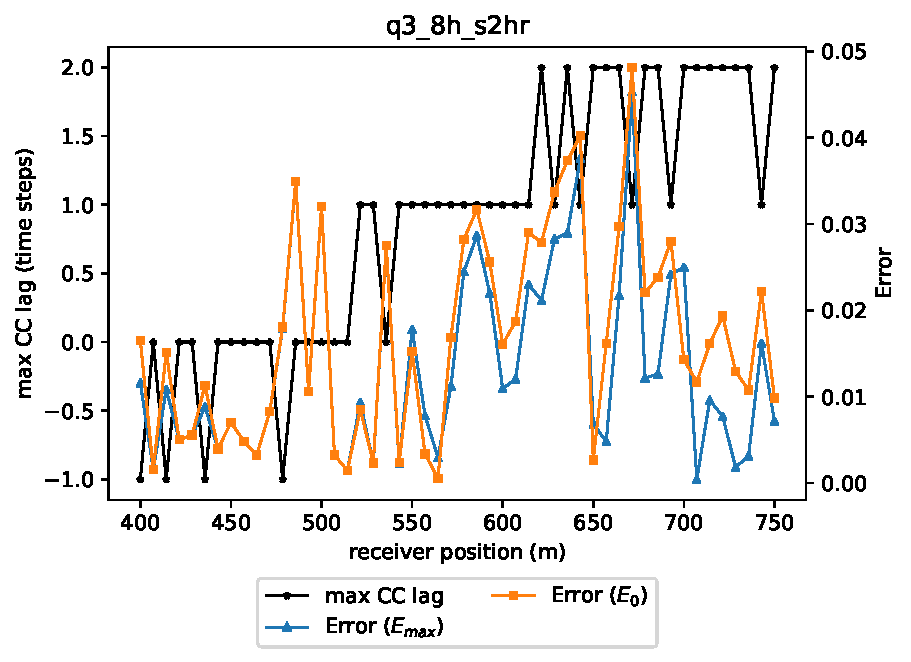
\includegraphics[width=8cm, height=6cm]{Thesis_Edith/figures/layered_model/layer_waves/Err_q3_8h_s2hr.pdf}
			   \caption{}
				%\label{fig:3.7b}
		\end{subfigure}
 
	\caption{Layered model: Maximum cross correlation lag and errors for each receiver seismogram for 2 GFEM solutions with 3 plane wave directions and mesh size of $8h$. (a) For the GFEM solution with source size of $8h$. (b) For the GFEM solution with source size of $2h$}
	\label{fig:3.20}
\end{figure}

%gFem error
 \begin{figure}[h!]
 		\centering
		\begin{subfigure}{8cm}
				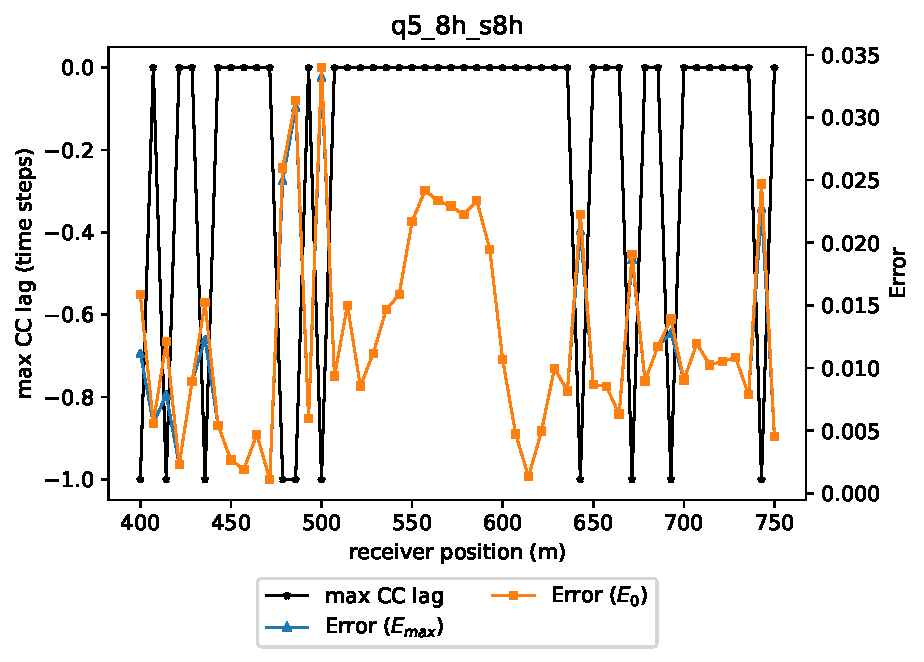
\includegraphics[width=8cm, height=6cm]{Thesis_Edith/figures/layered_model/layer_waves/Err_q5_8h_s8h.pdf}
			     \caption{}
				%\label{fig:3.7a}
		\end{subfigure}
        \hspace{0.25cm}	
		\begin{subfigure}{8cm}
				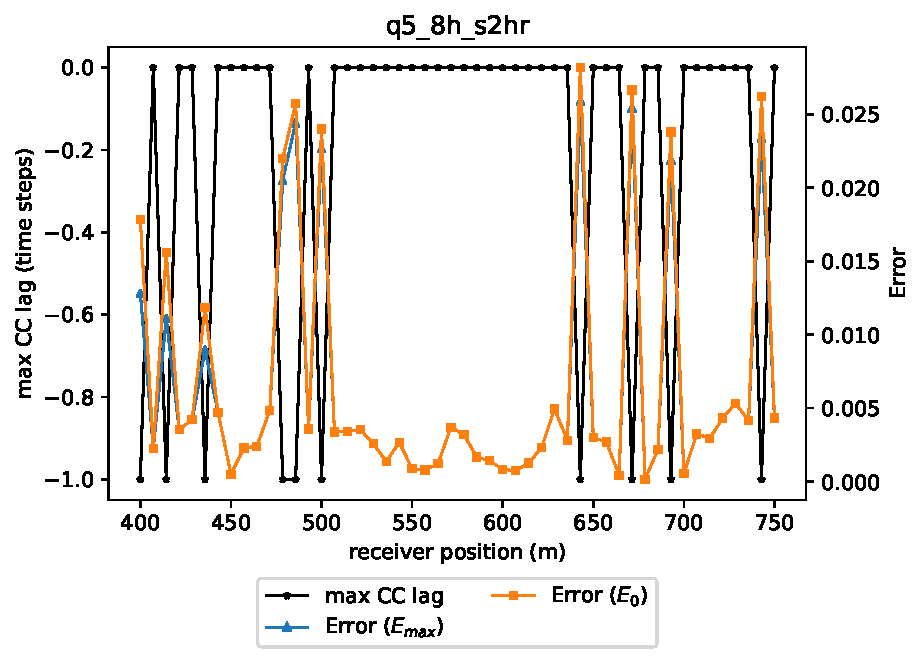
\includegraphics[width=8cm, height=6cm]{Thesis_Edith/figures/layered_model/layer_waves/Err_q5_8h_s2hr.pdf}
			   \caption{}
				%\label{fig:3.7b}
		\end{subfigure}
 
	\caption{Layered model: Maximum cross correlation lag and errors for each receiver seismogram for 2 GFEM solutions with 5 plane wave directions and mesh size of $8h$. (a) For the GFEM solution with source size of $8h$. (b) For the GFEM solution with source size of $2h$}
	\label{fig:3.21}
\end{figure}

Figure \ref{fig:3.22} shows the mean error versus relative simulation time and standard deviation for the FEM solutions and for various GFEM cases. According to theses results, the GFEM cases are faster than the FEM reference solution and than the FEM solution in a mesh of $2h$ inclusive. The fastest solutions belong to the GFEM solutions implemented with 3 plane waves directions, due to their lower number of DOFs.
Regarding the mean error, all but one GFEM solution present lower error than any of the FEM solutions is coarser meshes of $2h$ and $4h$, and the GFEM solutions with 5 plane waves directions presents the 2 lowest errors. 
For the standard deviation, results trends resemble those of the mean error vs time, with lower standard deviation corresponding to the GFEM cases except one and with the 2 lowest standard deviation corresponding to the GFEM solutions with 5 plane wave directions. Observe as well that the accuracy of GFEM results improve with the smallest source size. 


% Time v error
%*******
 \begin{figure}[h!]
 		\centering
		\begin{subfigure}{8cm}
				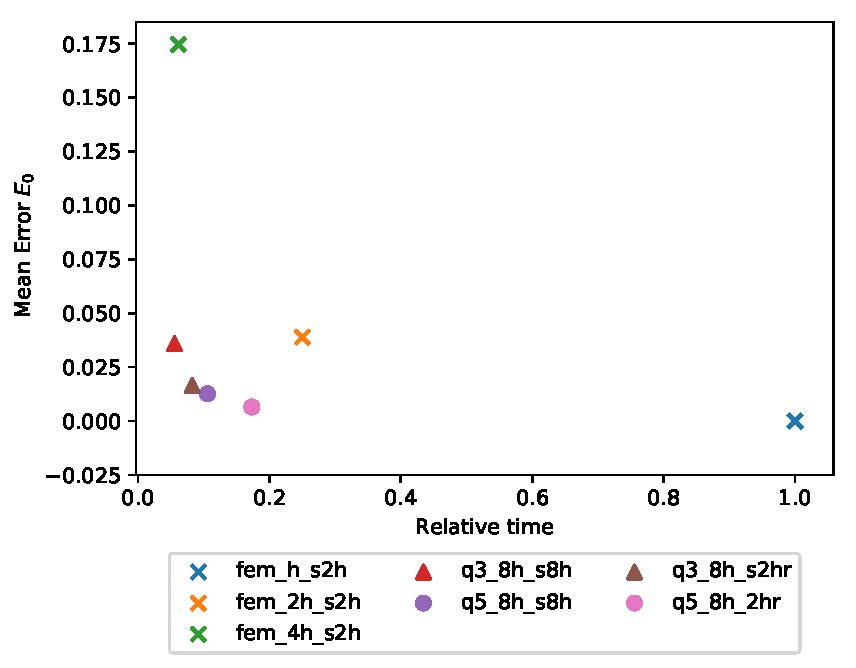
\includegraphics[width=8cm, height=6cm]{Thesis_Edith/figures/layered_model/layer_waves/MeanError_time_layered.pdf}
			     \caption{}
				%\label{fig:3.7a}
		\end{subfigure}
        \hspace{0.25cm}	
		\begin{subfigure}{8cm}
				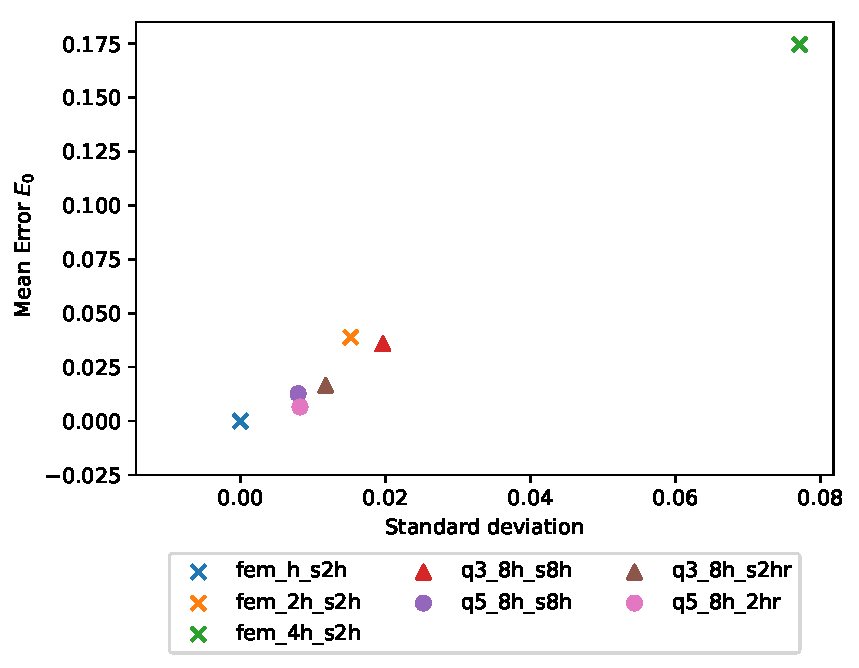
\includegraphics[width=8cm, height=6cm]{Thesis_Edith/figures/layered_model/layer_waves/MeanError_std_layered.pdf}
			   \caption{}
				%\label{fig:3.7b}
		\end{subfigure}
 
	\caption{Layered model: Mean error vs relative time and standard deviation for various FEM and GFEM cases. (a) Mean error vs relative time. (b) Mean error vs standard deviation.}
	\label{fig:3.22}
\end{figure}


 \clearpage
% New section: Scattering Model
%*******************************
\section{Case 3: Model with Karst Inclusion (Scattering Model)}
The model for this example is as shown in Figure \ref{fig:3.23}. This model is similar to the layered model, however for this case the top layer velocity is half of that in the layered model, to simulate a poor consolidated layer. This model also presents a karst inclusion which is assumed to be full of water. The main goal of this simulation model is to show the capability of the GFEM approach to combine flexible local refinement with its computational efficiency. 

 In this model, The source is located at the same position as in the layered model: -50 m in the vertical coordinate and 400 m in the horizontal coordinate and has a frequency of 40 Hz. There are 100 receivers placed close to the surface and span from 50 m to 750 m in the horizontal coordinates. Table \ref{table:3.2} shows the velocity, wavelengths and wavenumbers for each of the geological features present in the model. It also shows the number cells per wavelength for different mesh sizes.

 \begin{figure}[h!]
	\centering
	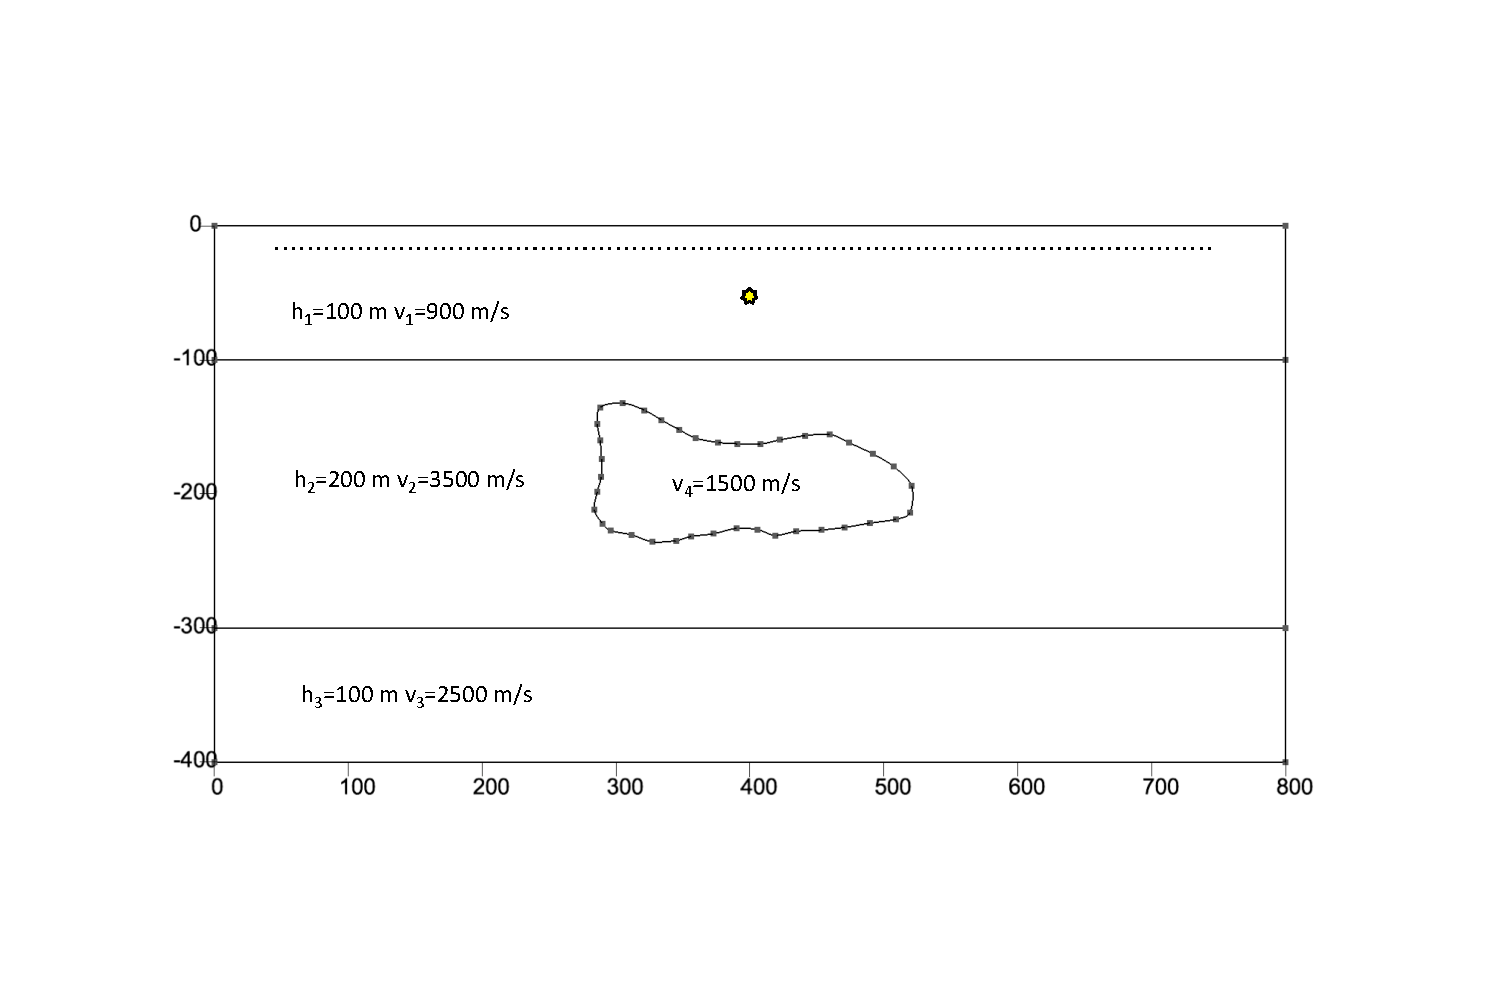
\includegraphics[width=14cm, height=7cm]{Thesis_Edith/figures/scattering/scatter_source.pdf}
	\caption{Scattering model with a seismic source in the first layer (yellow star) and a horizontal array of 100 receivers close to surface as depicted by the dotted line.}
	\label{fig:3.23}
\end{figure}

%table
\begin{table}[h!]
\footnotesize
\centering
    \begin{tabular}{|c|m{1.5cm}|m{2cm}|m{2cm}|m{1cm}| m{0.8cm}|m{0.8cm}|m{0.8cm}|m{0.8cm}|}
      \hline
      \multirow{2}{*}{Feature} &
      \multirow{2}{1.5cm}{Velocity (m/s)} &
      \multirow{2}{2cm}{Wavelength \quad $\lambda$ (m)} &
      \multirow{2}{2cm}{Wavenumber  k (m$^{-1}$)} &
         \multicolumn{5}{m{5cm}|}{Number of cells per wavelength in a mesh size of :} \\
         & & &  &$h/2$ & $h$ & $2h$ & $4h$ & $8h$ \\
      \hline
      1 & 900 & 22.5 & 0.28 & 28.8 & 14.4 & 7.2 & 3.6 & 1.8\\
      \hline
      2 & 3500 & 87.5 & 0.07 & 112 & 56 & 28 & 14 & 7\\
      \hline
      3 & 2500 & 62.5 & 0.10 & 80 & 40 & 20 & 10 & 5\\
      \hline
      4 & 1500 & 37.5 & 0.17 & 48 & 24 & 12 & 6 & 3\\
       \hline
    \end{tabular}
    \caption{Scattering model: Table showing the velocity, wavelength and wavenumber for each geological feature in the model, as well as the number cells per wavelength in different mesh sizes. Source frequency is 40 Hz and $h=$1.5625 m}
    \label{table:3.2}
\end{table}

For the reference solution, I use a similar mesh as in Figure \ref{fig:3.24}, but for this case the mesh size is $h$ except for the top layer, for which a mesh size of $h/2$ is used. I use similar coarser meshes - of sizes $2h$ and $4h$ and top layer mesh sizes of $h$ and $2h$ correspondingly -  to run two additional FEM cases. 
For the GFEM simulation cases I use two mesh configurations: one as shown in Figure \ref{fig:3.25}, with a background mesh size of $8h$ and of size $4h$ for the top layer. The second mesh  is as in Figure \ref{fig:3.26}, which is similar to the first one but with additional refinement around the karst feature. The goal of this additional refinement is to conform better to the karst geometrical shape, and as consequence obtain a more accurate simulation. For all the GFEM cases the wave number used for the plane wave enrichments is 0.28 m$^{-1}$, calculated by dividing the source radial frequency by the lowest geological feature velocity (900 m/s).

%Meshes
 \begin{figure}[h!]
	\centering
	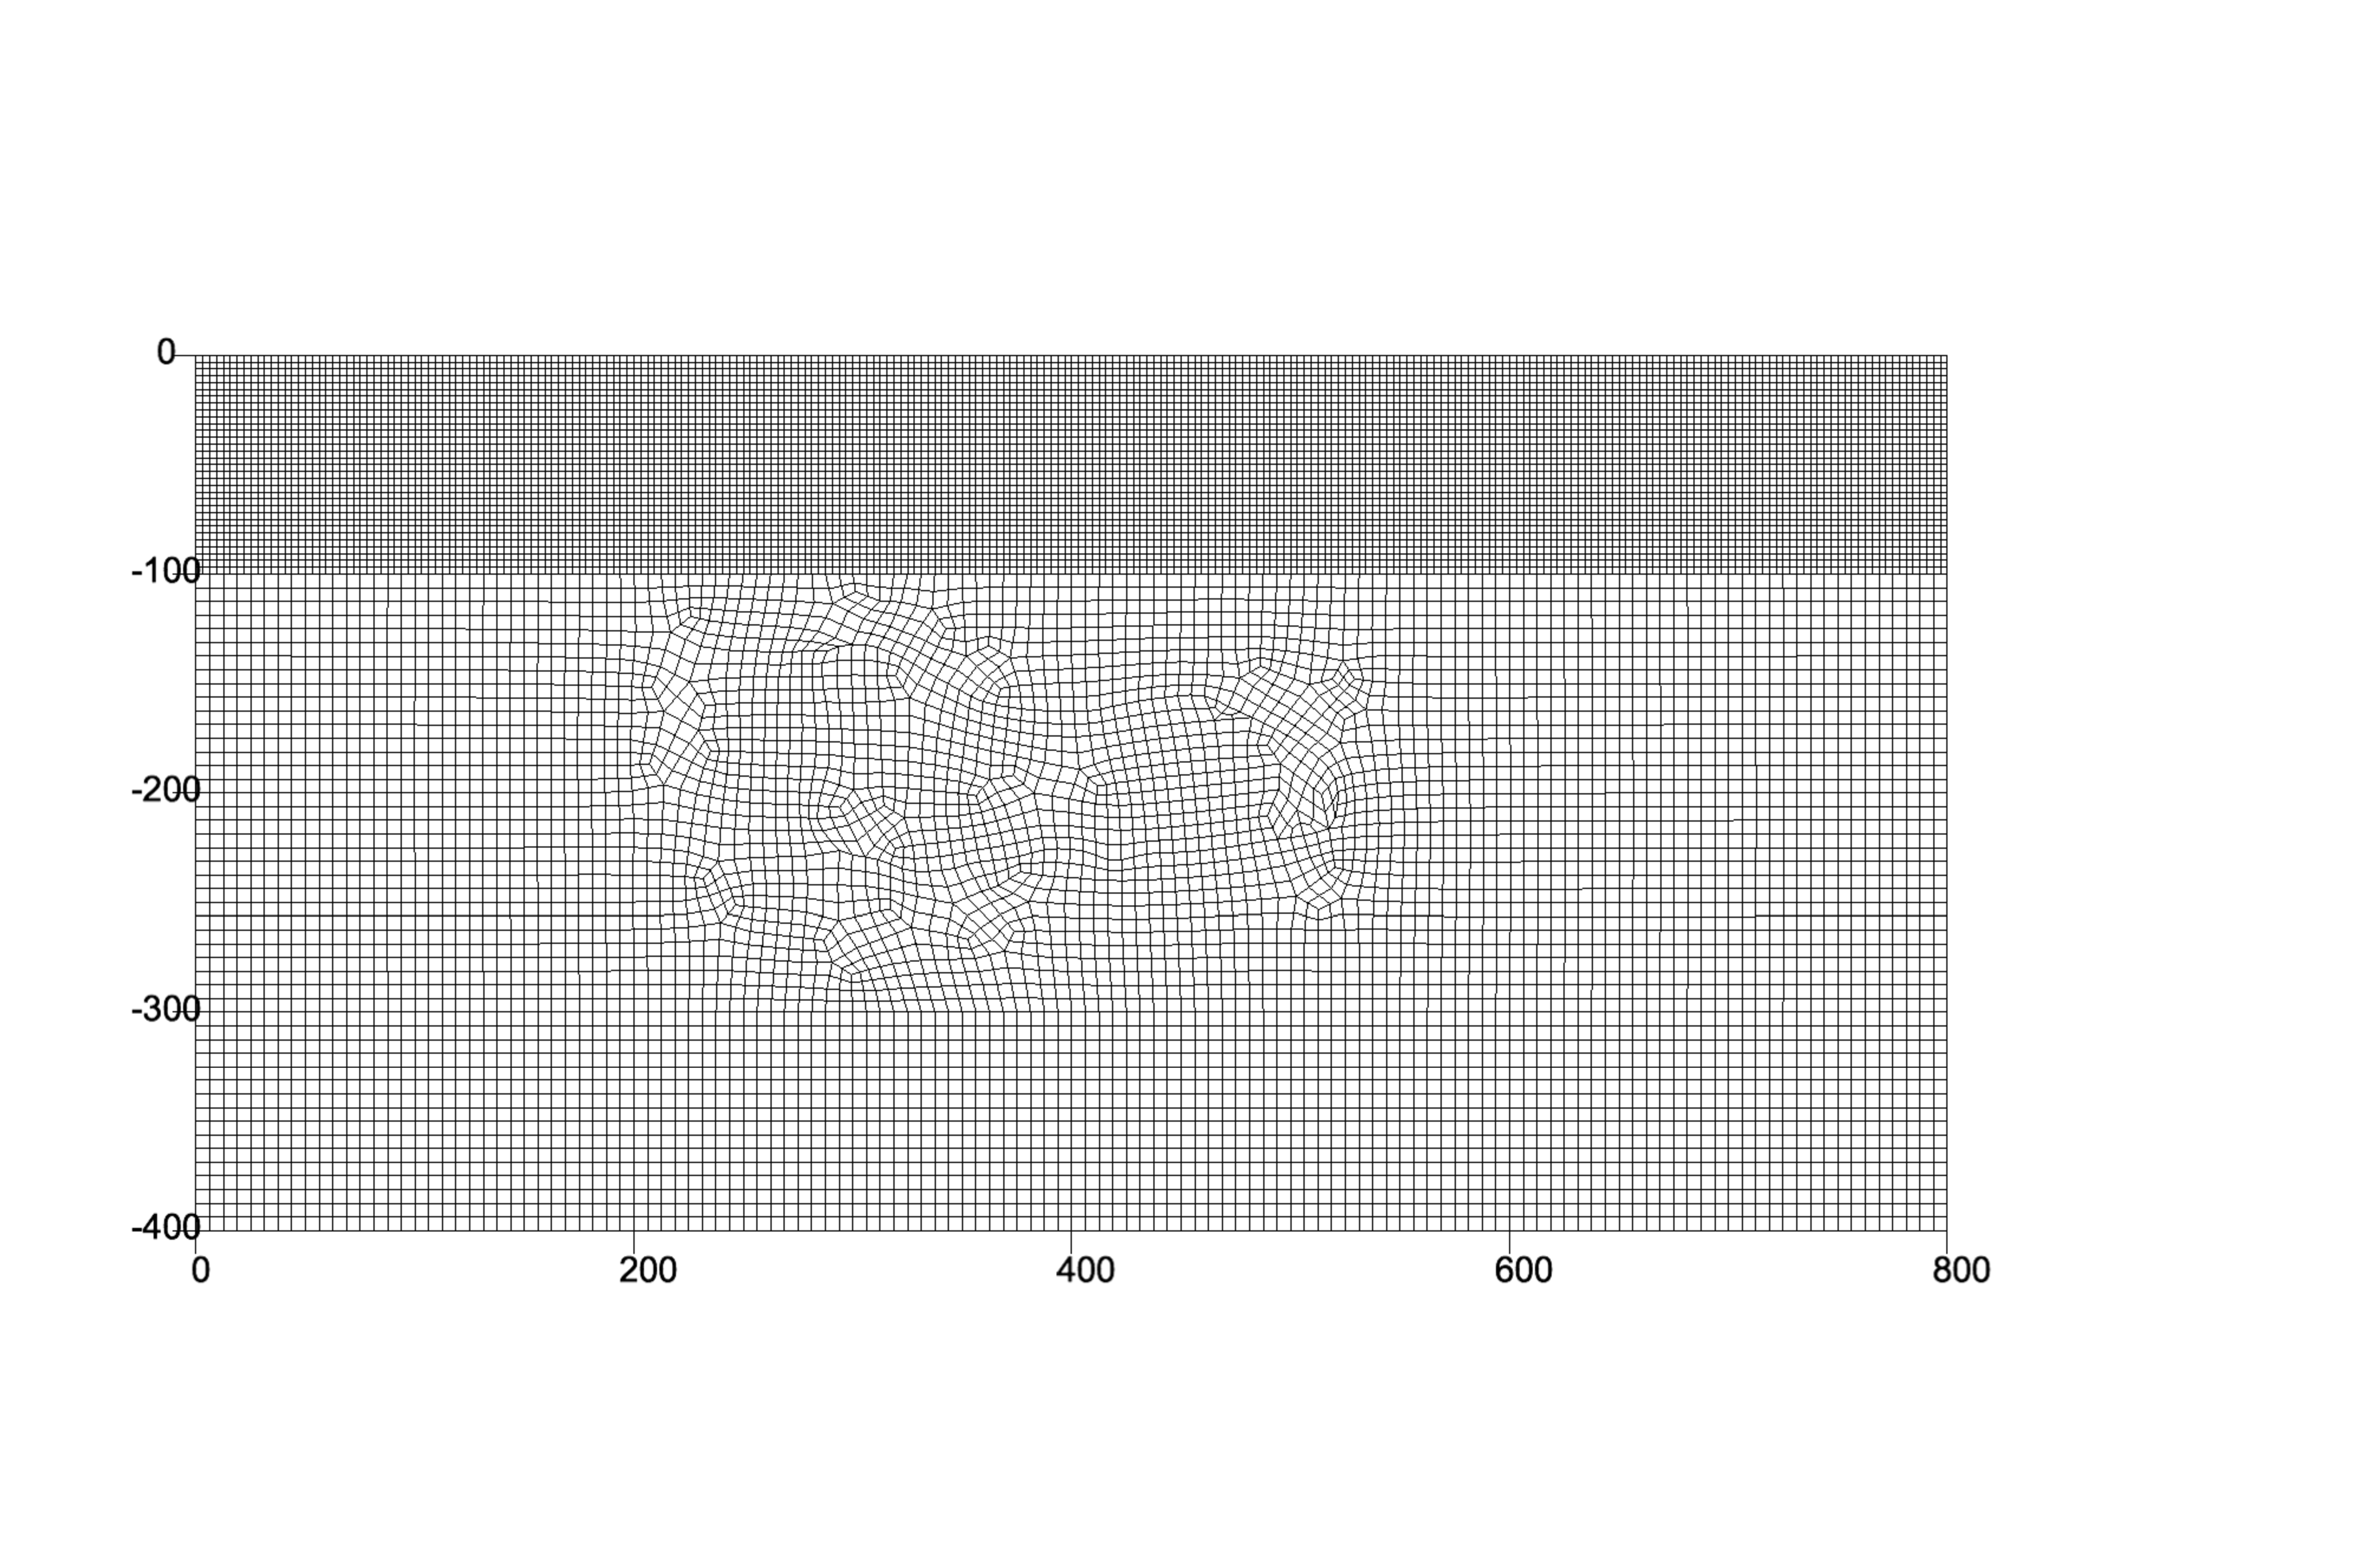
\includegraphics[width=16cm, height=8cm]{Thesis_Edith/figures/scattering/mesh_ref_mr4_v2.pdf}
	\caption{Scattering model: Example of one of the meshes used for the  standard FEM simulations. The original mesh with grid size of $4h$ is subdivided in half ($2h$) at the top layer.}
	\label{fig:3.24}
\end{figure}

 \begin{figure}[h!]
	\centering
	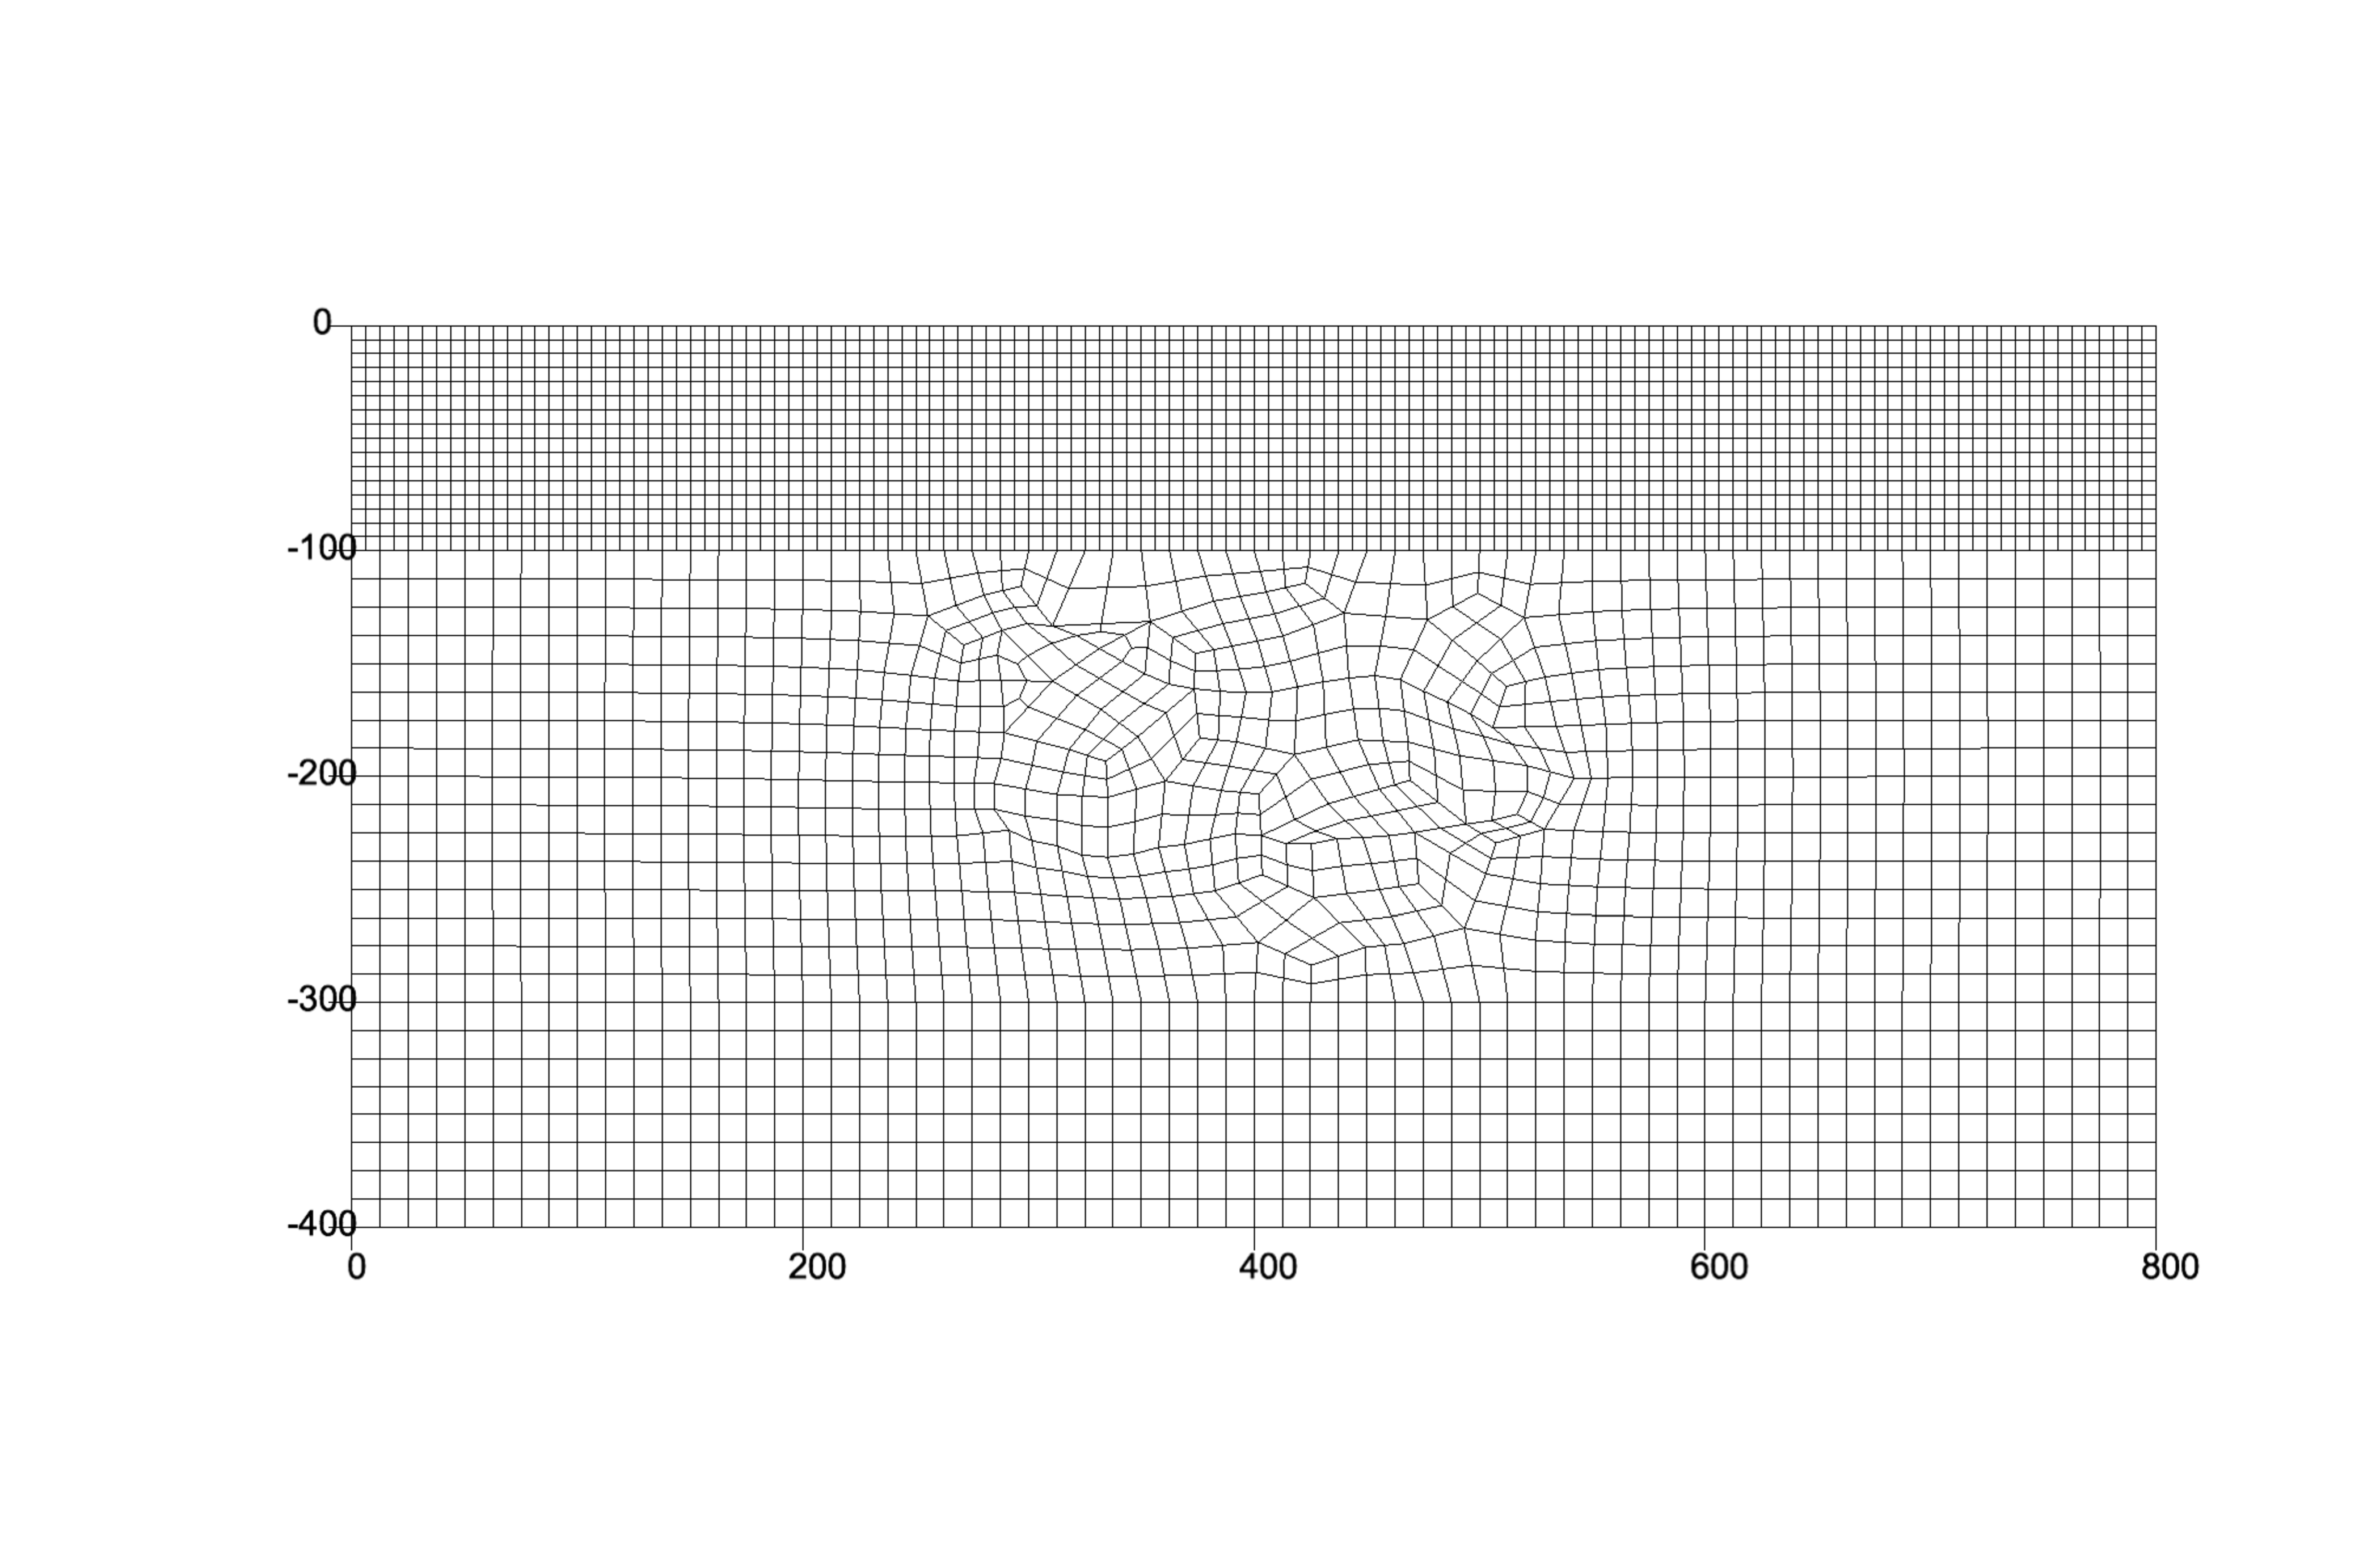
\includegraphics[width=16cm, height=8cm]{Thesis_Edith/figures/scattering/mesh_ref_mr3_v2.pdf}
	\caption{Scattering model: Example of a type of mesh used for the GFEM simulations. The original mesh with grid size of $8h$ is subdivided in half ($4h$) at the top layer.}
	\label{fig:3.25}
\end{figure}

 \begin{figure}[h!]
	\centering
	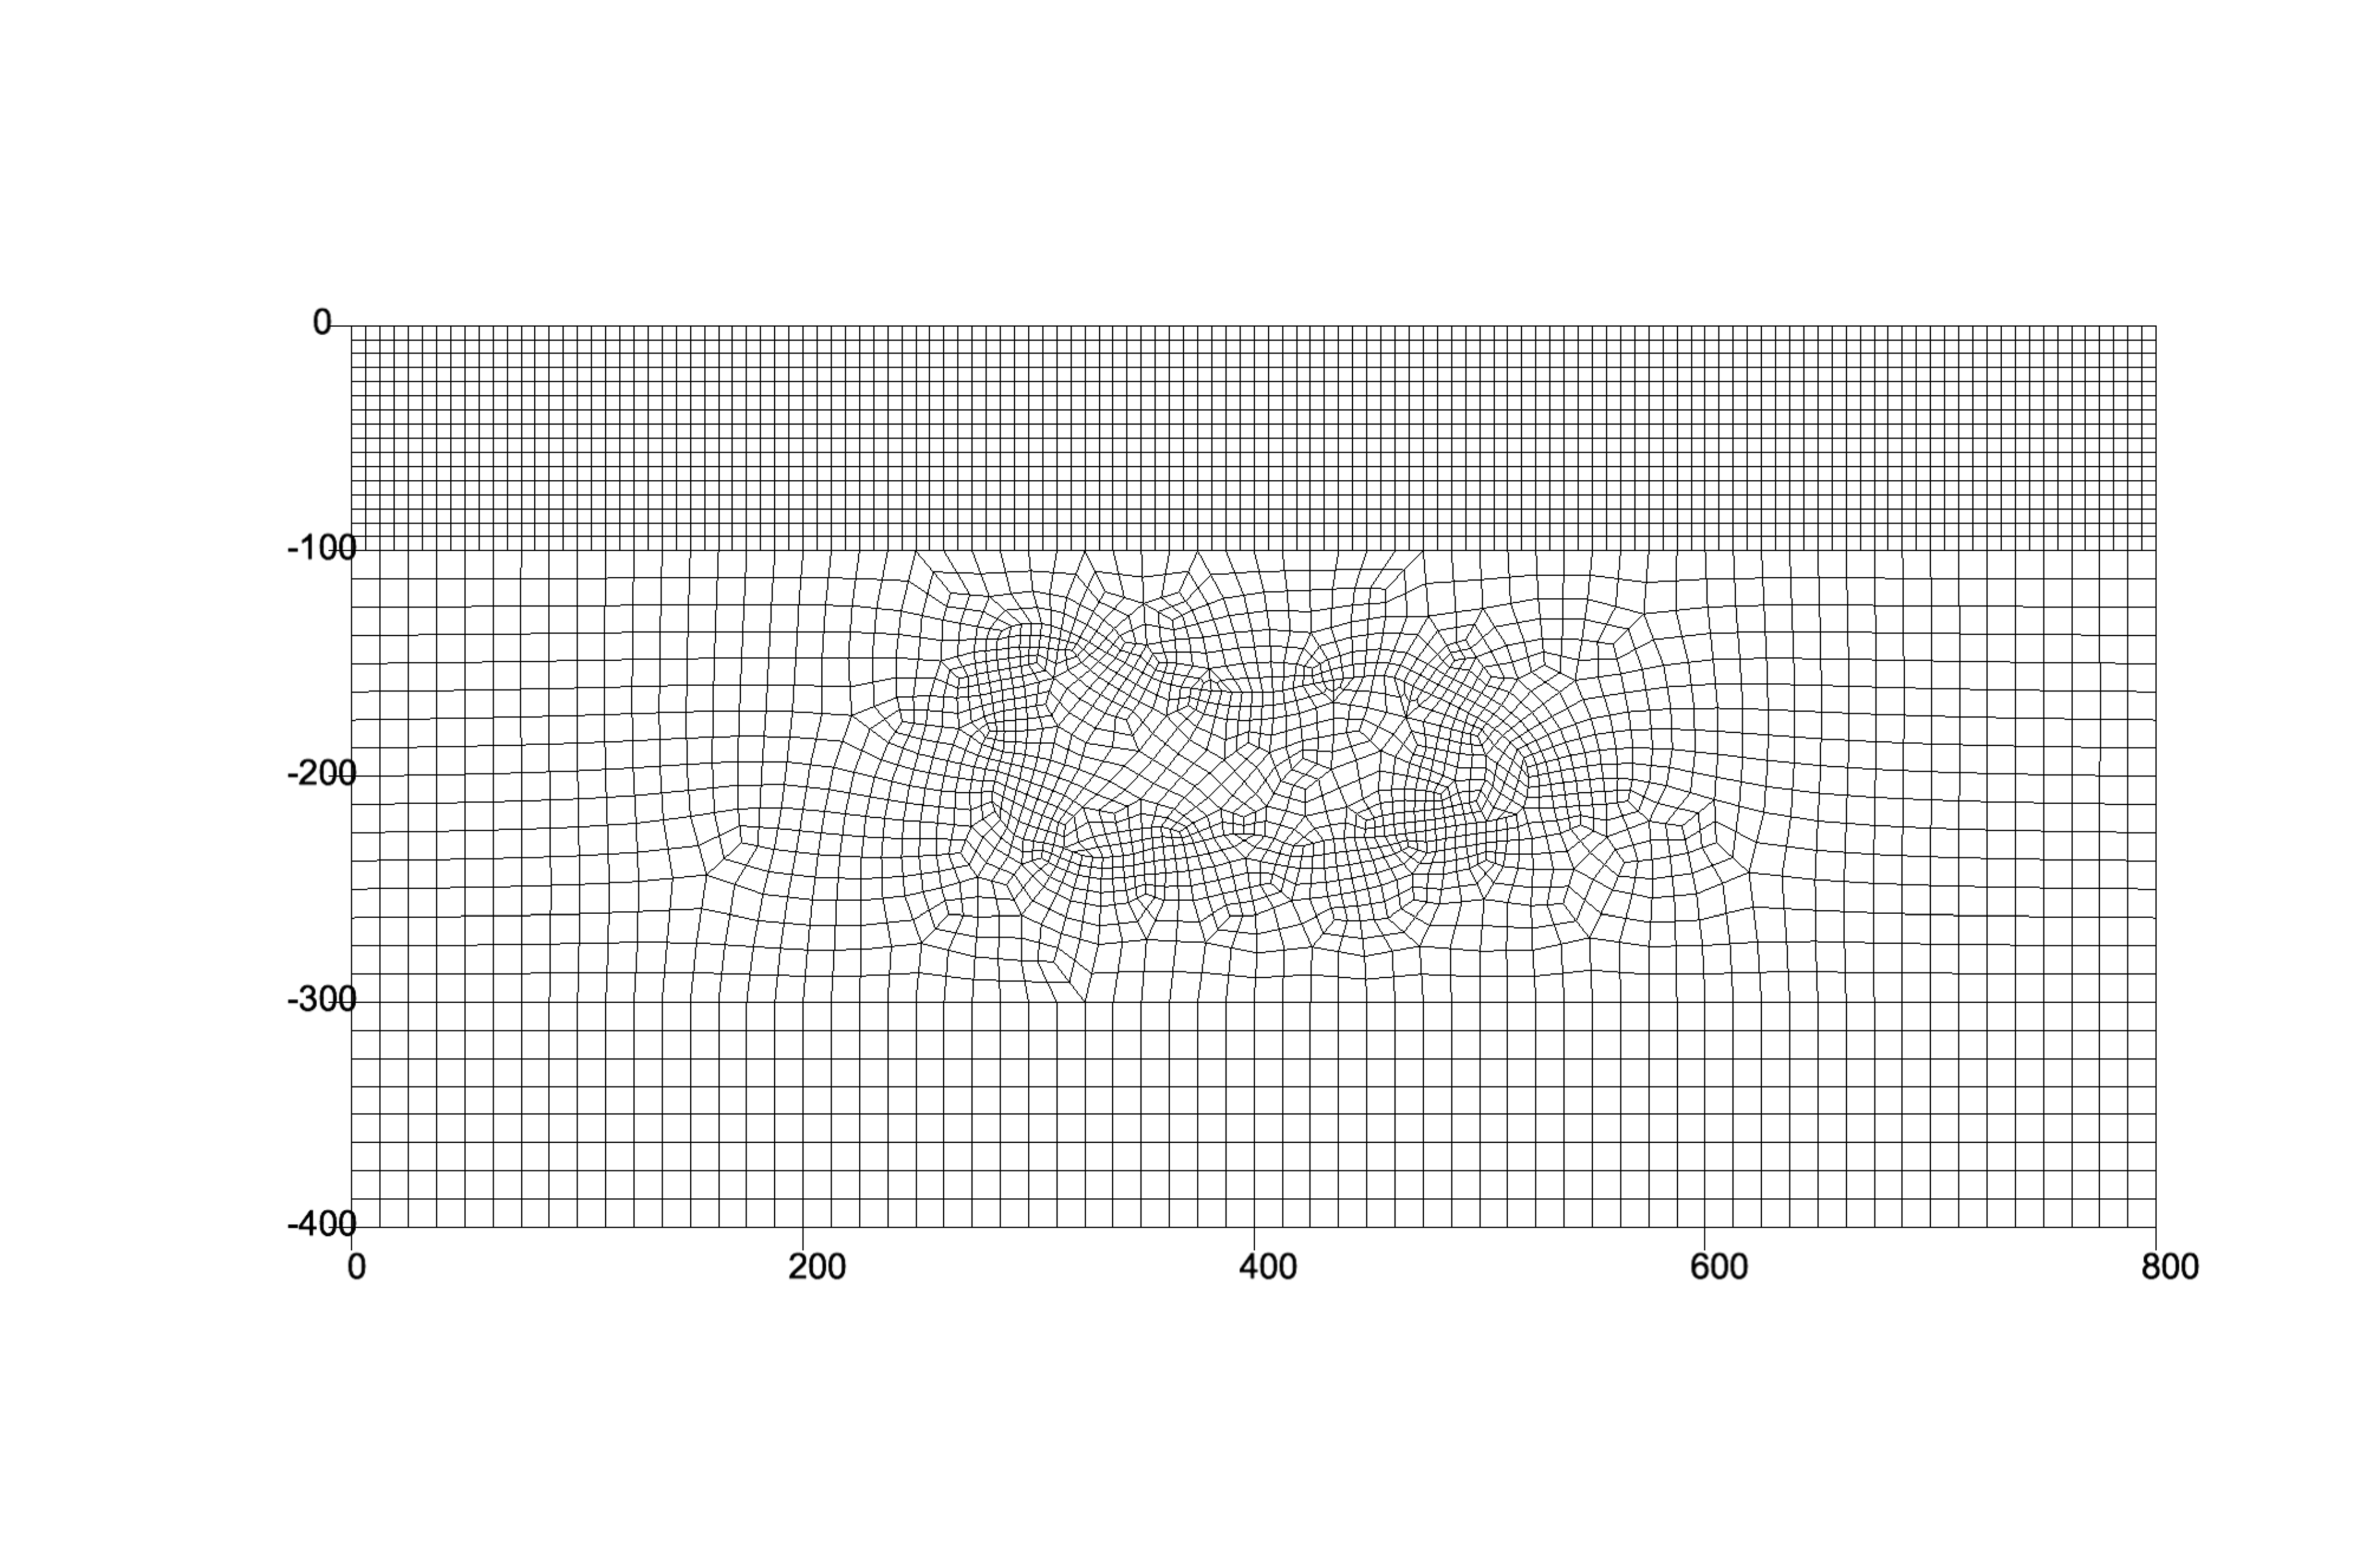
\includegraphics[width=16cm, height=8cm]{Thesis_Edith/figures/scattering/meshr_ref_v2.pdf}
	\caption{Scattering model: Example of a type of mesh used for GFEM simulations. This mesh is similar to the mesh in Figure \ref{fig:3.25} with additional refinement around the karst inclusion.}
	\label{fig:3.26}
\end{figure}

%******
\clearpage
Figure \ref{fig:3.27} shows the seismogram of the shot gather for the reference solution. Prominent features are the direct wave, the reflection at the bottom of the top layer and the multiple scattering effects produced by the karst inclusion.
%shot gather
 \begin{figure}[h!]
	\centering
	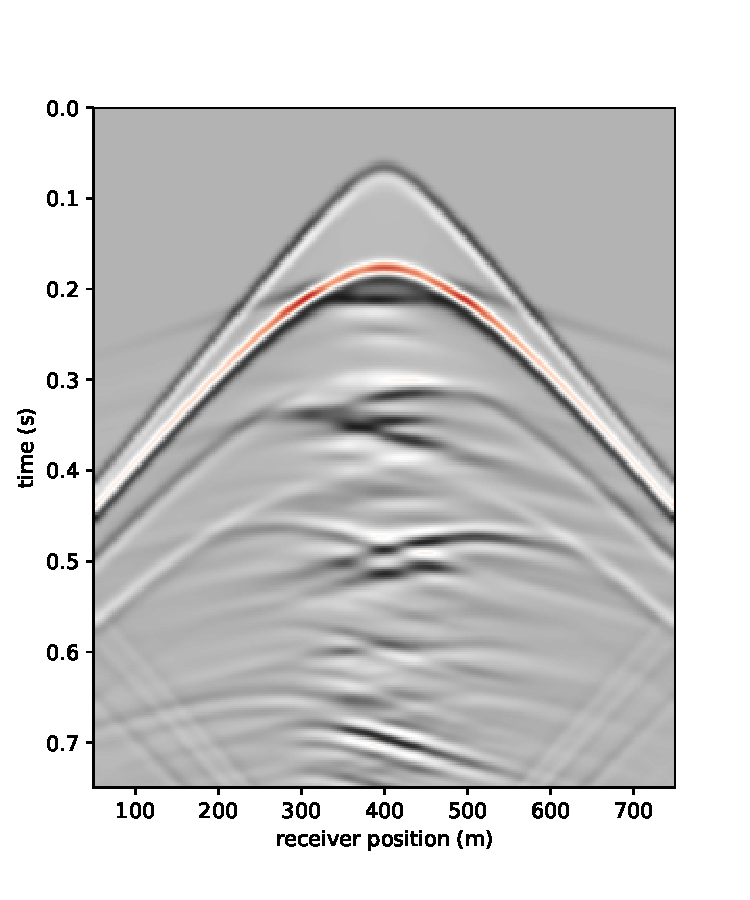
\includegraphics[width=10cm, height=13cm]{Thesis_Edith/figures/scattering/scat_waves/seismogram_scattering.pdf}
	\caption{Scattering model: Seismograms of the shot gather for the reference solution. Divergence coefficient is 2.5}
	\label{fig:3.27}
\end{figure}

%******
\clearpage
Figure \ref{fig:3.28} shows the seismograms for the reference solution and 2 additional FEM simulation cases with coarser meshes for receivers placed at 156.1 m and 580.3 m in the horizontal coordinate. As expected simulation results deteriorate in accuracy as the mesh is coarsened when compared to the reference solution.

Figures \ref{fig:3.29} and \ref{fig:3.30} show the seismograms for the reference solution and GFEM simulation cases with 5 plane wave directions obtained for receivers placed at 156.1 m and 580.3 m in the horizontal coordinate respectively. In both of these figures I compare the effect of source size and of the additional refinement around the karst feature. As found in the layered model example, a decrease in source size improves the accuray of the simulation result. The additional refinement around the karst feature also improves the match of reflections coming at later times with the reference solution as pointed by the arrows in the figures.

Figure \ref{fig:3.31} shows the seismograms for the reference solution and for a GFEM simulation case with 3 plane wave directions obtained for receivers placed at 156.1 m and 580.3 m in the horizontal coordinate respectively. I this case I use a mesh as in figure \ref{fig:3.24} with no additional refinement around the karst inclusion. This is the same mesh used for the FEM case with the coarsest mesh. However, when compared the results of GFEM  with that of the corresponding FEM in figure  \ref{fig:3.28}, the GFEM outcomes are much more accurate.


%fem traces
 \begin{figure}[h!]
 		\centering
		\begin{subfigure}{8cm}
				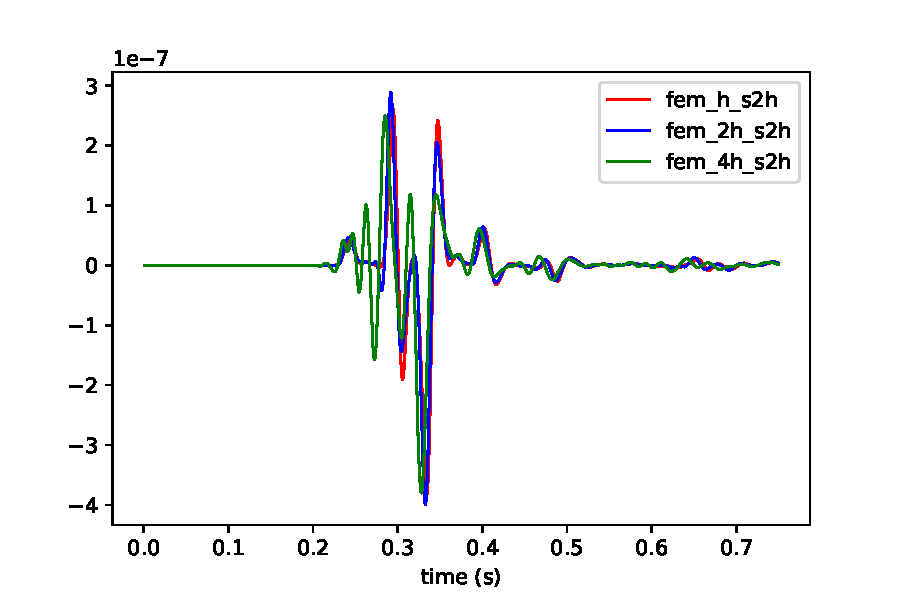
\includegraphics[width=8cm, height=5.5cm]{Thesis_Edith/figures/scattering/scat_waves/fem_scat_tr15.pdf} 
			     \caption{}
				%\label{fig:3.7a}
		\end{subfigure}
        \hspace{0.25cm}	
		\begin{subfigure}{8cm}
				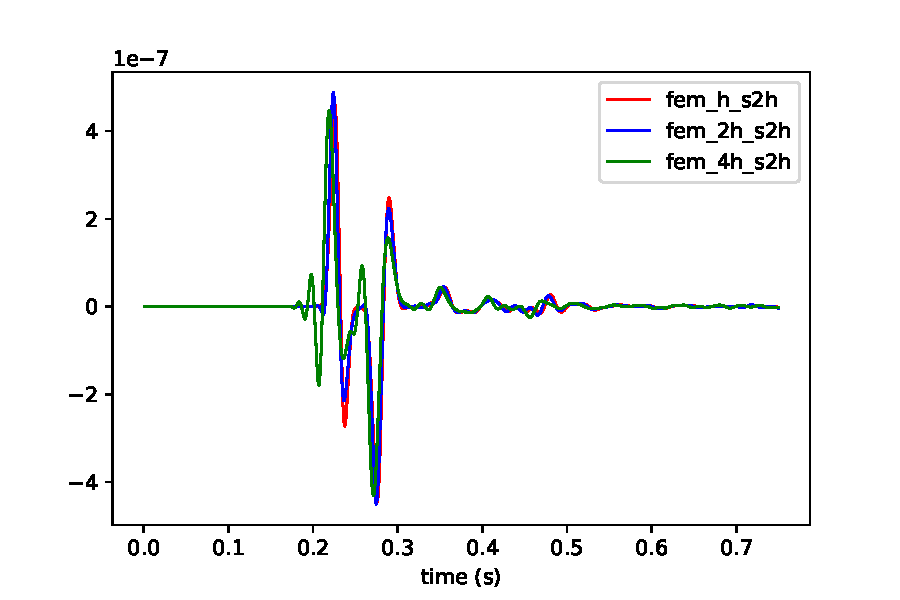
\includegraphics[width=8cm, height=5.5cm]{Thesis_Edith/figures/scattering/scat_waves/fem_scat_tr75.pdf}
			   \caption{}
				%\label{fig:3.7b}
		\end{subfigure}
 
	\caption{Scattering model: Seismograms of the reference solution in a mesh size of $h$ and $h/2$ at the top layer and for 2 additional FEM solutions in coarser meshes. (a) Seimograms from a receiver located at 156.1 m in the horizontal coordinate. (b) Seimograms from a receiver located at 580.3 m in the horizontal coordinate.}
	\label{fig:3.28}
\end{figure}

%gfem traces
 \begin{figure}[h!]
 		\centering
		\begin{subfigure}{8cm}
				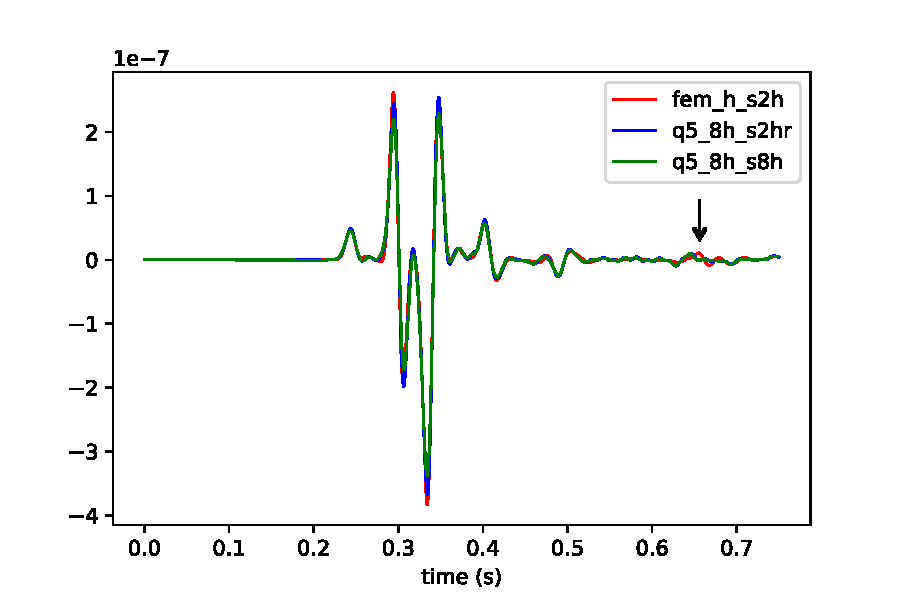
\includegraphics[width=8cm, height=5.5cm]{Thesis_Edith/figures/scattering/scat_waves/gfem_scat_tr15_v2.pdf} 
			     \caption{}
				%\label{fig:3.7a}
		\end{subfigure}
        \hspace{0.25cm}	
		\begin{subfigure}{8cm}
				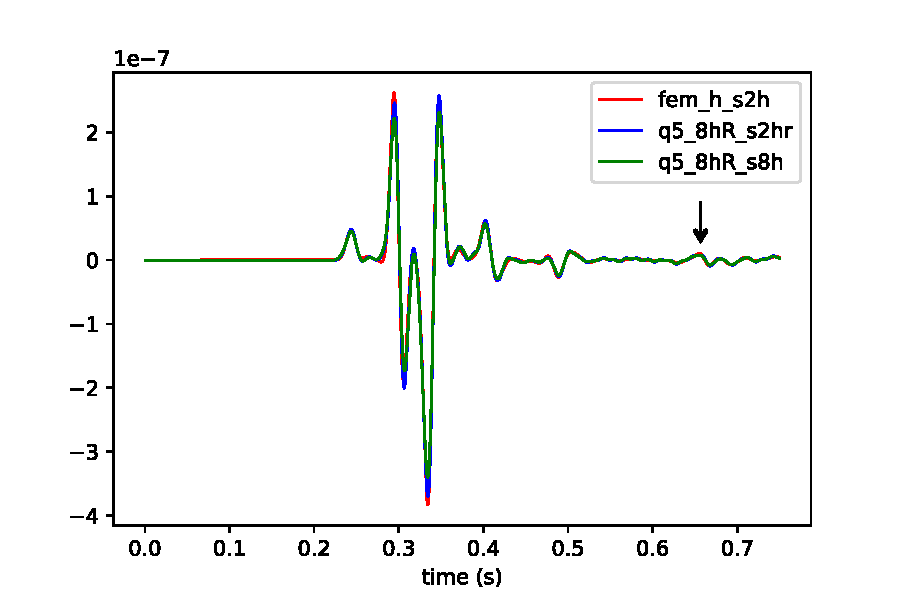
\includegraphics[width=8cm, height=5.5cm]{Thesis_Edith/figures/scattering/scat_waves/gfemr_scat_tr15_v2.pdf}
			   \caption{}
				%\label{fig:3.7b}
		\end{subfigure}
 
	\caption{Scattering model: Seismograms from a receiver located at 156.1 m in the horizontal coordinate for the reference solution and  GFEM solutions obtained   with 5 plane wave directions and with  a source radius of $2h$ and $8h$. (a) Seismograms showing GFEM solutions obtained in a mesh as in Figure \ref{fig:3.25}. (b) Seismograms showing GFEM solutions obtained in a mesh as in Figure \ref{fig:3.26}. Arrows show the difference in the GFEM seismograms.}
	\label{fig:3.29}
\end{figure}

 \begin{figure}[h!]
 		\centering
		\begin{subfigure}{8cm}
				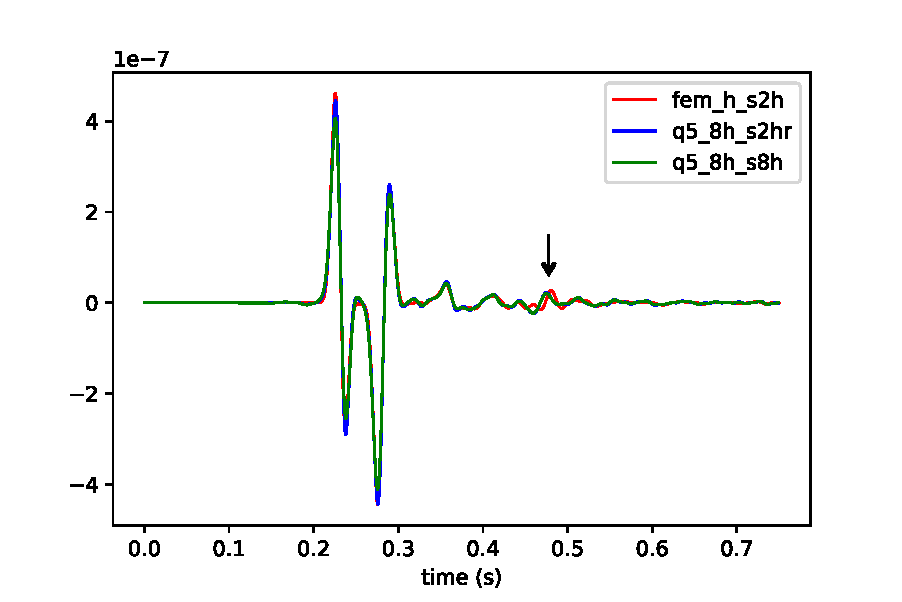
\includegraphics[width=8cm, height=5.5cm]{Thesis_Edith/figures/scattering/scat_waves/gfem_scat_tr75_v2.pdf} 
			     \caption{}
				%\label{fig:3.7a}
		\end{subfigure}
        \hspace{0.25cm}	
		\begin{subfigure}{8cm}
				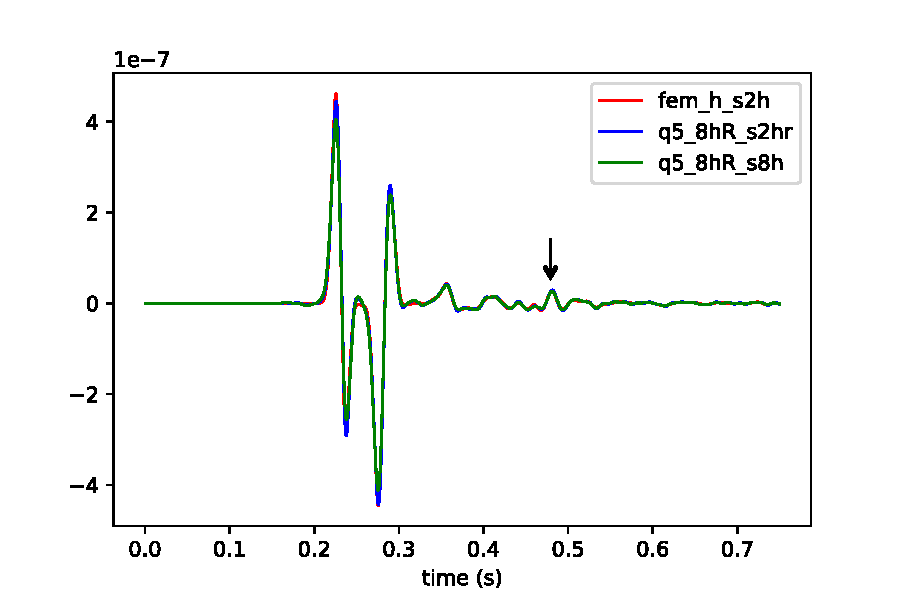
\includegraphics[width=8cm, height=5.5cm]{Thesis_Edith/figures/scattering/scat_waves/gfemr_scat_tr75_v2.pdf}
			   \caption{}
				%\label{fig:3.7b}
		\end{subfigure}
 
	\caption{Scattering model: Seismograms from a receiver located at 580.3 m in the horizontal coordinate for the reference solution and  GFEM solutions obtained  with  with 5 plane wave directions and a source radius of $2h$ and $8h$. (a) Seismograms showing GFEM solutions obtained in a mesh as in Figure \ref{fig:3.25}. (b) Seismograms showing GFEM solutions obtained in a mesh as in Figure \ref{fig:3.26}. Arrows show the difference between the GFEM seismograms in (a) and (b).}
	\label{fig:3.30}
\end{figure}

 \begin{figure}[h!]
 		\centering
		\begin{subfigure}{8cm}
				\includegraphics[width=8cm, height=5.5cm]{Thesis_Edith/figures/scattering/scat_waves/gfem3_scat_tr15.pdf}
			     \caption{}
				%\label{fig:3.7a}
		\end{subfigure}
        \hspace{0.25cm}	
		\begin{subfigure}{8cm}
				\includegraphics[width=8cm, height=5.5cm]{Thesis_Edith/figures/scattering/scat_waves/gfem3_scat_tr75.pdf}
			   \caption{}
				%\label{fig:3.7b}
		\end{subfigure}
 
	\caption{Scattering model: Scattering model: Seismograms from a receiver located at 580.3 m in the horizontal coordinate for the reference solution and a GFEM solution obtained with 3 plane wave directions, in a mesh of size  $4h$ and $2h$ at the top layer and with a source radius of $2h$.}
	\label{fig:3.31}
\end{figure}

\clearpage
 Figure \ref{fig:3.32} presents the maximum cross correlation lag and two error types with respect to the reference solution, calculated for the two FEM simulations across the 100 receiver seismograms. As noted in the layered model error analysis, the maximum cross correlation lag and the associated errors increase as the receivers get further away from the source center (400 m). This effect is the greatest for the FEM with the coarsest mesh. As also noted before, the error related to the maximum cross correlation ($E_{max}$) is lower than the one related to the zero lag cross correlation ($E_0$) and their difference increases as the source-receiver offset increases. These results show not only the numerical error as the seismic wave travels further away from the source but also the dispersion error caused by increasing the mesh size.
 
 Figures \ref{fig:3.33} and \ref{fig:3.34} show the maximum cross correlation lag and two error types with respect to the reference solution for several GFEM cases obtained with 5 plane wave directions. Each of these figures compare the effect of refinement around the karst inclusion as source size is kept constant. Note that in both figures, there are results spiking up from the average.  These spikes correspond to receivers located at 467.2 m and 474.2 m. I examine possible causes of these anomalous outputs in the appendix. Disregarding the two irregular outputs in all figures, the effect of the additional refinement around the karstic feature is practically imperceptible, however the effect of decreasing source size is evident, causing a decrease in the errors. Overall, as mentioned for the layered model, errors are consistent across the 100 receivers, showing little dispersion effect. 
 Figure \ref{fig:3.35} shows the maximum cross correlation lag and two error types with respect to the reference solution for an additional GFEM case obtained with 3 plane wave directions. For this case, a minimum error lag of -1 time step exist for the receivers at both ends and in general the errors are consistent in average across the 100 receivers, increasing slightly as the receivers get further away from the center of the source. 
 
%fem error
 \begin{figure}[h!]
 		\centering
		\begin{subfigure}{8cm}
				\includegraphics[width=8cm, height=5.5cm]{Thesis_Edith/figures/scattering/scat_waves/Err_fem_2h.pdf}
			     \caption{}
				%\label{fig:3.7a}
		\end{subfigure}
        \hspace{0.25cm}	
		\begin{subfigure}{8cm}
				\includegraphics[width=8cm, height=5.5cm]{Thesis_Edith/figures/scattering/scat_waves/Err_fem_4h.pdf}
			   \caption{}
				%\label{fig:3.7b}
		\end{subfigure}
 
	\caption{Scattering model: Maximum cross correlation lag and errors for 100 receiver seismograms for the 2 FEM cases. (a) For the FEM solution with mesh size of $2h$ and $h$ at the top layer. (b) For the FEM solution with mesh size of $4h$ and $2h$ at the top layer.}
	\label{fig:3.32}
\end{figure}

%gfem error
 \begin{figure}[h!]
 		\centering
		\begin{subfigure}{8cm}
				\includegraphics[width=8cm, height=5.5cm]{Thesis_Edith/figures/scattering/scat_waves/Err_q5_8h_s8h.pdf}
			     \caption{}
				%\label{fig:3.7a}
		\end{subfigure}
        \hspace{0.25cm}	
		\begin{subfigure}{8cm}
				\includegraphics[width=8cm, height=5.5cm]{Thesis_Edith/figures/scattering/scat_waves/Err_q5_8hR_s8h.pdf}
			   \caption{}
				%\label{fig:3.7b}
		\end{subfigure}
 
	\caption{Scattering model: Maximum cross correlation lag and errors for 100 receiver seismograms for 2 GFEM cases with 5 plane wave directions and source size of $8h$. (a) For the GFEM solution with mesh as in Figure \ref{fig:3.25}. (b) For the GFEM solution with mesh as in Figure \ref{fig:3.26}, which adds refinement around the karst feature.}
	\label{fig:3.33}
\end{figure}

 \begin{figure}[h!]
 		\centering
		\begin{subfigure}{8cm}
				\includegraphics[width=8cm, height=5.5cm]{Thesis_Edith/figures/scattering/scat_waves/Err_q5_8h_s2hr.pdf}
			     \caption{}
				%\label{fig:3.7a}
		\end{subfigure}
        \hspace{0.25cm}	
		\begin{subfigure}{8cm}
				\includegraphics[width=8cm, height=5.5cm]{Thesis_Edith/figures/scattering/scat_waves/Err_q5_8hR_s2hr.pdf}
			   \caption{}
				%\label{fig:3.7b}
		\end{subfigure}
 
	\caption{Scattering model: Maximum cross correlation lag and errors for 100 receiver seismograms for 2 GFEM cases with 5 plane wave directions and source size of $2h$. (a) For the GFEM solution with mesh as in Figure \ref{fig:3.25}. (b) For the GFEM solution with mesh as in Figure \ref{fig:3.26}, which adds refinement around the karst feature.}
	\label{fig:3.34}
\end{figure}


 \begin{figure}[h!]
	\centering
	\includegraphics[width=10cm, height=6cm]{Thesis_Edith/figures/scattering/scat_waves/Err_q3_4h_s2hr.pdf}
	\caption{Scattering model: Maximum cross correlation lag and errors for 100 receiver seismograms for a GFEM solution with 3 plane wave directions, mesh size of $4h$ and $2h$ at the top layer, and with source size of $2h$.}
	\label{fig:3.35}
\end{figure}

%*****
\clearpage
Figure \ref{fig:3.36} shows the mean error versus relative simulation time and standard deviation for the FEM and GFEM cases. Regarding GFEM results,the fastest times correspond to the GFEM solutions with 5 plane wave directions, the coarsest mesh and the biggest source size ($8h$), but the smallest errors correspond for the GFEM solutions with the smallest source size($2h$), either for 3 or 5 plane wave directions. In general the effect of the additional refinement around the karst feature is very mild and can be noticed as a slightly lower standard deviation. 

%Error vs time
 \begin{figure}[h!]
 		\centering
		\begin{subfigure}{8cm}
				\includegraphics[width=8cm, height=5.5cm]{Thesis_Edith/figures/scattering/scat_waves/MeanError_time_scat.pdf}
			     \caption{}
				%\label{fig:3.7a}
		\end{subfigure}
        \hspace{0.25cm}	
		\begin{subfigure}{8cm}
				\includegraphics[width=8cm, height=5.5cm]{Thesis_Edith/figures/scattering/scat_waves/MeanError_std_scat.pdf}
			   \caption{}
				%\label{fig:3.7b}
		\end{subfigure}
 
	\caption{Scattering model: Mean error vs relative time and standard deviation for various FEM and GFEM cases. (a) Mean error vs relative time. (b) Mean error vs standard deviation. }
	\label{fig:3.36}
\end{figure}

%*****
\clearpage

% New section: Topographic Model
%*******************************
\section{Case 4: Model with Topography (Topographic Model)}
The model for this example is as shown in Figure \ref{fig:3.37}. This model is similar to the scattering model, but for this case a topographic relief is present on the top layer with the same velocity (900 m/s).
In this simulation, the objective is to show the GFEM capability to handle the meshing of geometrically complex domain boundaries while keeping its computational efficiency.

In this model, the source is located in the same position as in the previous models: -50 m in the vertical direction and 400 m in the horizontal coordinate, and has a frequency of 40 Hz. The receiver array geometrical configuration is the same as in the scattering model: 100 receivers deployed very close to zero depth and spanning from 50 to 750 m in the horizontal coordinates. Table \ref{table:3.3} shows the velocity, wavelengths and wavenumber for the top layer. It also shows the number number of cells per wavelength in different refined mesh sizes. Table \ref{table:3.4} shows similar information for the remaining geological features.

For this case, I apply a free boundary condition at the curvy top layer boundary to simulate the multiple chaotic reflections produced by waves bouncing back and forth between the top and bottom boundaries of this first layer with topography.
To find a reference solution I use a similar mesh as in Figure \ref{fig:3.38}, but for this case the mesh sizes were $h$ and $0.6 h$ for the top layer with relief. I used similar but coarser meshes - of sizes $2h$ and $4h$ with top layer mesh sizes of $0.6 (2h)$ and $0.6 (4h)$ correspondingly- to run two additional FEM cases. For the GFEM simulations, I use the mesh configuration as in Figure \ref{fig:3.38} - for the GFEM case with 3 plane wave directions; and the meshes as in Figures \ref{fig:3.39} and \ref{fig:3.40} for the GFEM cases with 5 plane wave directions. For all the GFEM cases the wave number used is 0.28 m$^{-1}$, calculated by dividing the source radial frequency (2$\pi$ 40) by the lowest geological feature velocity (900 m/s).

 \begin{figure}[h!]
	\centering
	\includegraphics[width=14cm, height=7cm]{Thesis_Edith/figures/topo/topo_source.pdf}
	\caption{Seismic model including both topography and karst inclusion. The seismic source is located in the first layer (yellow star) and a horizontal array of 100 receivers is located close to zero depth as depicted by the dotted line.}
	\label{fig:3.37}
\end{figure}

%table
\begin{table}[h!]
\footnotesize
\centering
    \begin{tabular}{|c|m{1.5cm}|m{2cm}|m{2cm}|m{1cm}| m{1.2cm}|m{1.2cm}|m{1.2cm}|m{1.2cm}|}
      \hline
      \multirow{2}{*}{Feature} &
      \multirow{2}{1.5cm}{Velocity (m/s)} &
      \multirow{2}{2cm}{Wavelength \quad $\lambda$ (m)} &
      \multirow{2}{2cm}{Wavenumber  k (m$^{-1}$)} &
         \multicolumn{4}{m{6 cm}|}{Number of cells per wavelength in a mesh size of :} \\
         & &  &  & $0.6 \, (h)$ & $ 0.6 \, (2h)$ & $ 0.6 \, (4h) $ & $ 0.6 \, (8h)$ \\
      \hline
      1 & 900 & 22.5 & 0.28 & 24 & 12 & 6  & 3 \\
     \hline
    \end{tabular}
    \caption{Topographic model: Table showing the velocity, wavelength and wavenumber for the top layer in the model, as well as the number cells per wavelength in different mesh sizes. Source frequency is 40 Hz and $h=$1.5625 m}
    \label{table:3.3}
\end{table}

%table
\begin{table}[h!]
\footnotesize
\centering
    \begin{tabular}{|c|m{1.5cm}|m{2cm}|m{2cm}|m{1cm}| m{0.8cm}|m{0.8cm}|m{0.8cm}|m{0.8cm}|}
      \hline
      \multirow{2}{*}{Feature} &
      \multirow{2}{1.5cm}{Velocity (m/s)} &
      \multirow{2}{2cm}{Wavelength \quad $\lambda$ (m)} &
      \multirow{2}{2cm}{Wavenumber  k (m$^{-1}$)} &
         \multicolumn{4}{m{5cm}|}{Number of cells per wavelength in a mesh size of :} \\
         & & &  & $h$ & $2h$ & $4h$ & $8h$ \\
      \hline
      2 & 3500 & 87.5 & 0.07 & 56 & 28 & 14 & 7\\
      \hline
      3 & 2500 & 62.5 & 0.10 & 40 & 20 & 10 & 5\\
      \hline
      4 & 1500 & 37.5 & 0.17 & 24 & 12 & 6 & 3\\
       \hline
    \end{tabular}
    \caption{Topographic model: Table showing the velocity, wavelength and wavenumber for the remaining geological features in the model, as well as the number cells per wavelength in different mesh sizes. Source frequency is 40 Hz and $h=$1.5625 m}
    \label{table:3.4}
\end{table}
%mesh
 \begin{figure}[h!]
	\centering
	\includegraphics[width=14cm, height=7cm]{Thesis_Edith/figures/topo/topo_mesh_4hv2.pdf}
	\caption{Topographic model: Example of one of the meshes used for the standard FEM simulations. Mesh size is $0.6 (4h)$ in the top layer with topographic relief and $4h$ in the rest of the model.}
	\label{fig:3.38}
\end{figure}

 \begin{figure}[h!]
	\centering
	\includegraphics[width=14cm, height=7cm]{Thesis_Edith/figures/topo/topo_meshr_8hv2.pdf}
	\caption{Topographic model: Example of one of the meshes used for the GFEM simulations. Mesh size is $0.6 (8h)$ in the top layer with topographic relief and $8h$ in the rest of the model.}
	\label{fig:3.39}
\end{figure}

 \begin{figure}[h!]
	\centering
	\includegraphics[width=14cm, height=7cm]{Thesis_Edith/figures/topo/topo_meshr_refv2.pdf}
	\caption{Topographic model: Example of one of meshes used for the GFEM simulations. This mesh is similar to the one in Figure \ref{fig:3.39} but with additional refinement around the karst inclusion.}
	\label{fig:3.40}
\end{figure}

%**********
\clearpage
Figure \ref{fig:3.41} shows the seismograms for the shot gather configuration shown in Figure \ref{fig:3.37} obtained for the reference solution. Observe that the seismograms are saturated with multiple reflections produced by waves bouncing between the top and bottom boundaries of the first layer. These reflections hinder the visualization of other reflections produced at the boundaries of the other two deeper layers and of the karst inclusion.

%shot gather
 \begin{figure}[h!]
	\centering
	\includegraphics[width=10cm, height=13cm]{Thesis_Edith/figures/topo/topo_waves/seismogram_topo.pdf}
	\caption{Topographic model: Seismograms for the shot gather configuration as in Figure \ref{fig:3.37} obtained for the reference solution. Divergence coefficient is 1.5.}
	\label{fig:3.41}
\end{figure}

%*******
\clearpage
%traces
Figure \ref{fig:3.42} shows the seismograms for the reference solution and 2 additional FEM simulations obtained in coarser meshes at a receiver located at 580.3 m in the horizontal coordinate. Notice the complex waveform reflections and that this additional FEM solutions cannot reproduce various complicated details of the reference waveform.

Figure \ref{fig:3.43} shows the seismograms for the reference solution and GFEM simulations obtained with 5 plane wave directions at a receiver located at 580.3 m in the horizontal coordinate. Sub-figures (a) and (b) correspond to meshes without and with refinement around the karstic feature respectively. Notice that since the multiple reflections at the top layer overshadow other incoming reflections, there is no visible improvement of the additional refinement performed around the karst feature as it was evident in the case of the scattering model.

Figure \ref{fig:3.44} shows the seismograms for the reference solution and GFEM simulations obtained with 3 plane wave directions at a receiver located at 580.3 m in the horizontal coordinate. This GFEM solution was obtained in a mesh as shown in Figure \ref{fig:3.38}, which is a finer mesh than the ones used for the GFEM solutions as in Figure \ref{fig:3.43}. Notice the improvement in the match of the waveforms with the reference solution. However, this increase in accuracy due to a decrease in mesh size affects the efficiency of the simulation time as more DOFs are needed. See Figure \ref{fig:3.49} for details in the simulation time and errors.

%fem traces
 \begin{figure}[h!]
 		\centering
		\begin{subfigure}{8cm}
				\includegraphics[width=8cm, height=5.5cm]{Thesis_Edith/figures/topo/topo_waves/fem_topo_tr75.pdf}
			     \caption{}
				%\label{fig:3.7a}
		\end{subfigure}
        \hspace{0.25cm}	
		\begin{subfigure}{8cm}
				\includegraphics[width=8cm, height=5.5cm]{Thesis_Edith/figures/topo/topo_waves/fem_topo2h_tr75.pdf}
			   \caption{}
				%\label{fig:3.7b}
		\end{subfigure}
 
	\caption{Topographic model: Seismograms for a receiver at 580.3 m in the horizontal coordinate, for the FEM reference solution with a mesh of size $h$ and $0.6 h$ at the top layer, and  additional FEM solutions obtained in coarser meshes. (a) Seismograms showing the reference solution and 2 additional FEM solutions. (b) Same as (a) but disregarding the FEM solution in the coarsest mesh.}
	\label{fig:3.42}
\end{figure}


%gfem traces
 \begin{figure}[h!]
 		\centering
		\begin{subfigure}{8cm}
				\includegraphics[width=8cm, height=5.5cm]{Thesis_Edith/figures/topo/topo_waves/gfem_topo_tr75.pdf}
			     \caption{}
				%\label{fig:3.7a}
		\end{subfigure}
        \hspace{0.25cm}	
		\begin{subfigure}{8cm}
				\includegraphics[width=8cm, height=5.5cm]{Thesis_Edith/figures/topo/topo_waves/gfemr_topo_tr75.pdf}
			   \caption{}
				%\label{fig:3.7b}
		\end{subfigure}
 
	\caption{Topographic model: Seismograms for a receiver at 580.3 in the horizontal coordinate, for the FEM reference solution and various GFEM cases obtained with 5 plane wave directions and source radius of $8h$ and $2h$. (a) Seismograms for the reference solution and 2 GFEM cases obtained in a mesh as in Figure \ref{fig:3.39}. (b) Seismograms for the reference solution and 2 GFEM cases obtained in a mesh as in Figure \ref{fig:3.40}, which presents refinement around the karst feature.}
	\label{fig:3.43}
\end{figure}

%traces gfem3
 \begin{figure}[h!]
	\centering
	\includegraphics[width=8cm, height=6cm]{Thesis_Edith/figures/topo/topo_waves/gfem3_topo_tr75.pdf}
	\caption{Topographic model: Seismograms for a receiver at 580.3 in the horizontal coordinate of the FEM reference solution and a GFEM case obtained with 3 plane wave directions, mesh  as in Figure \ref{fig:3.38} and source radius of $8h$ and $2h$.}
	\label{fig:3.44}
\end{figure}

%error
\clearpage
Figure \ref{fig:3.45} present the maximum cross correlation lag and two error types with respect to the reference solution, calculated for two FEM simulations across the 100 receivers of the model. As with the results for the previous models, the lag and errors increase as the receivers get further away from the source center in the horizontal coordinate (400 m), with the greatest effect for the FEM with the coarsest mesh. For this FEM case (sub-figure (a)), the maximum cross correlation lag goes up to 18 time steps and errors take values as high as more than 0.6. As discussed before, these errors evidence the effect of dispersion which worsen as grid size becomes coarser. 

Figures \ref{fig:3.46} and Figure \ref{fig:3.47} present the maximum cross correlation lag and two error types with respect to the reference solution calculated for various GFEM simulations obtained with 5 plane wave directions across the 100 receivers of the model. For each figure, the corresponding sub-figures present results for meshes without and with additional mesh refinement around the karst feature, keeping source radius constant respectively. As mentioned before, the effect of the karst feature on the results are imperceptible. On the other hand, notice that the lag and errors do not vary much across the receivers, with the least errors corresponding to the GFEM cases with the smallest source radius. As already mentioned, these results show that despite the coarse mesh used, the enrichments implemented in the GFEM approach diminish dispersion effects, and that matching the source size to that of the reference solution further improves the accuracy of the outputs.

Figure \ref{fig:3.48} presents the maximum cross correlation lag and two error types with respect to the reference solution, calculated for a GFEM case obtained with 3 plane wave directions across the 100 receivers of the model. This is the GFEM solution obtained in the finest mesh of all GFEM cases, same mesh as the coarsest mesh used for the FEM cases. Notice that there is no lag present across all the receivers for the maximum cross correlation and the errors are comparable to those corresponding to the best solution of the GFEM cases with 5 plane wave directions. 


%error fem
 \begin{figure}[h!]
 		\centering
		\begin{subfigure}{8cm}
				\includegraphics[width=8cm, height=5.5cm]{Thesis_Edith/figures/topo/topo_waves/Err_fem_2h.pdf}
			     \caption{}
				%\label{fig:3.7a}
		\end{subfigure}
        \hspace{0.25cm}	
		\begin{subfigure}{8cm}
				\includegraphics[width=8cm, height=5.5cm]{Thesis_Edith/figures/topo/topo_waves/Err_fem_4h.pdf}
			   \caption{}
				%\label{fig:3.7b}
		\end{subfigure}
 
	\caption{Topographic model: Maximum cross correlation lag and errors for 100 receivers for 2 FEM cases. (a) For the FEM solution in a mesh size of $2h$ and $0.6 (2h)$ at the top layer. (b) For the FEM solution in a mesh size of $4h$ and $0.6 (4h)$ at the top layer. }
	\label{fig:3.45}
\end{figure}




%error gfem
 \begin{figure}[h!]
 		\centering
		\begin{subfigure}{8cm}
				\includegraphics[width=8cm, height=5.5cm]{Thesis_Edith/figures/topo/topo_waves/Err_q5_8h_s8h.pdf}
			     \caption{}
				%\label{fig:3.7a}
		\end{subfigure}
        \hspace{0.25cm}	
		\begin{subfigure}{8cm}
				\includegraphics[width=8cm, height=5.5cm]{Thesis_Edith/figures/topo/topo_waves/Err_q5_8hR_s8h.pdf}
			   \caption{}
				%\label{fig:3.7b}
		\end{subfigure}
 
	\caption{Topographic model: Maximum cross correlation lag and errors for 100 receivers for 2 GFEM cases with 5 plane wave directions and source radius of $8h$. (a) For the GFEM solution in a mesh as in Figure \ref{fig:3.39}. (b) For the GFEM solution in a mesh as in figure \ref{fig:3.40}, which adds refinement around the karst feature.}
	\label{fig:3.46}
\end{figure}

 \begin{figure}[h!]
 		\centering
		\begin{subfigure}{8cm}
				\includegraphics[width=8cm, height=5.5cm]{Thesis_Edith/figures/topo/topo_waves/Err_q5_8h_s2hr.pdf}
			     \caption{}
				%\label{fig:3.7a}
		\end{subfigure}
        \hspace{0.25cm}	
		\begin{subfigure}{8cm}
				\includegraphics[width=8cm, height=5.5cm]{Thesis_Edith/figures/topo/topo_waves/Err_q5_8hR_s2hr.pdf}
			   \caption{}
				%\label{fig:3.7b}
		\end{subfigure}
 
	\caption{Topographic model: Maximum cross correlation lag and errors for 100 receivers for 2 GFEM cases with 5 plane wave directions and source radius of $2h$. (a) For the GFEM solution in a mesh as in Figure \ref{fig:3.39}. (b) For the GFEM solution in a mesh as in figure \ref{fig:3.40}, which adds refinement around the karst feature.}
	\label{fig:3.47}
\end{figure}

%traces gfem3
 \begin{figure}[h!]
	\centering
	\includegraphics[width=8cm, height=6cm]{Thesis_Edith/figures/topo/topo_waves/Err_q3_4h_s2hr.pdf}
	\caption{Topographic model: Maximum cross correlation lag and errors for 100 receivers for a GFEM case with 3 plane wave directions in a mesh as in Figure \ref{fig:3.38}.}
	\label{fig:3.48}
\end{figure}

%*********
\clearpage
Figure \ref{fig:3.49} shows the mean error versus relative simulation time and standard deviation for the FEM and GFEM cases. Regarding GFEM results, the fastest time correspond to the case with 5 plane wave directions, coarse mesh without refinement around the karst inclusion and the biggest source size. Correspondingly, 3 GFEM cases present the samllest error, 2 of them with five plane wave directions and the smallest source size and the other one correspond to the GFEM case with 3 plane wave directions. These cases also show small standard deviation with the smallest one belonging to the GFEM case with 3 plane wave directions.



%error time
 \begin{figure}[h!]
 		\centering
		\begin{subfigure}{8cm}
				\includegraphics[width=8cm, height=5.5cm]{Thesis_Edith/figures/topo/topo_waves/MeanError_time_topo.pdf}
			     \caption{}
				%\label{fig:3.7a}
		\end{subfigure}
        \hspace{0.25cm}	
		\begin{subfigure}{8cm}
				\includegraphics[width=8cm, height=5.5cm]{Thesis_Edith/figures/topo/topo_waves/MeanError_std_topo.pdf}
			   \caption{}
				%\label{fig:3.7b}
		\end{subfigure}
 
	\caption{Topographic model: Mean error versus relative time and standard deviation for various FEM and GFEM cases. (a) Mean error vs relative time. (b) Mean error vs standard deviation.}
	\label{fig:3.49}
\end{figure}